\documentclass[oneside,a4paper,titlepage]{scrartcl}              % Format fuer Titelseite und Dokument (KOMA-Script)
\usepackage[left=2.5cm,right=2.5cm,top=3cm,bottom=3cm]{geometry} % Raender verkleinern fuer mehr Platz
\usepackage[ngerman]{babel}                                      % Sprache
\usepackage[utf8]{inputenc}                                      % Direkte Eingabe von Umlauten Dokument
\usepackage[T1]{fontenc}                                         % Silbentrennung auch bei Woertern mit Umlauten
\usepackage{graphicx}                                            % Bilder
\usepackage{listings}                                            % Aufzaehlungen
\usepackage{xcolor}                                              % Farbgebung des Sourcodes
\usepackage{lmodern}                                             % Formatierung des Sourcecodes
\usepackage{longtable}                                           % Fuer mehrseitige Tabellen
\usepackage{booktabs}                                            % Fuer mehrseitige Tabellen
\usepackage{colortbl}                                            % Fuer farbige Zeilen/Reihen in Tabellen

% Formatierung fuer Sourcecode
\DeclareFontShape{OT1}{cmtt}{bx}{n}{<5><6><7><8><9><10><10.95><12><14.4><17.28><20.74><24.88>cmttb10}{}
\definecolor{eclipse-violet}{rgb}{0.50,0.0,0.46}
\definecolor{eclipse-green}{rgb}{0.25,0.50,0.37}
\definecolor{eclipse-blue}{rgb}{0.17,0.0,1.00}
\lstset{
  language=C++, % Fuer C++ Coding-Style
  showstringspaces=false,
  basicstyle=\ttfamily\small,
  keywordstyle=\bfseries\color{eclipse-violet},
  commentstyle=\color{eclipse-green},
  stringstyle=\color{eclipse-blue}
}

% Formatierung fuer Tabellen
\usepackage{tabularx}
\newcolumntype{L}[1]{>{\raggedright\arraybackslash}p{#1}} % L{1cm} fuer linksbuendig mit eigener Breitenangabe in Zentimetern
\newcolumntype{C}[1]{>{\centering\arraybackslash}p{#1}}   % C{2cm} fuer zentriert mit eigener Breitenangabe in Zentimetern
\newcolumntype{R}[1]{>{\raggedleft\arraybackslash}p{#1}}  % R{3cm} fuer rechtsbuendig mit eigener Breitenangabe in Zentimetern

% Fuer den automatischen Umbruch an einem Bindestrich, wie z.B. bei "Werkstueck-Sortieranlage", statt - die Zeichen "= verwenden

% Inhaltsverzeichnis anklickbar machen
\usepackage[pdftex]{hyperref}

% Beginn des Dokuments
\begin{document}

% Titelseite aufbauen
\titlehead{\flushright
\includegraphics[scale=.75]{imgs/HAW_logo.png}}
\subject{Software Engineering II\\Wintersemester 2014/2015}
\title{Requirements and Design Documentation}
\subtitle{Praktikums-Gruppe: 2.3}

% Titelseite: Autoren aufbauen
\author{
\begin{small}
  \begin{tabular}{|l|l|c|p{6cm}|}
    \hline
    \rowcolor{lightgray}\textbf{Name} & \textbf{Vorname} & \textbf{Matrikel-Nr.} & \textbf{E-Mail}\\
    \hline
    \rowcolor{white}Kirstein & Katja & 2125137 & katja.kirstein@haw-hamburg.de\\
    \hline
    Kowalka & Anne-Lena & 2081899 & anne-lena.kowalka@haw-hamburg.de\\
    \hline
    Triebe & Marian & 2124897 & marian.triebe@haw-hamburg.de\\
    \hline
    Winter & Eugen & 2081992 & eugen.winter@haw-hamburg.de\\
    \hline
  \end{tabular}
\end{small}
}

% Titelseite mit Datum und Version erstellen
\date{\today\thanks{Dokument-Version: 0.93}} % ! Hier die Versionsnummer an Versionshistorie anpassen !
\maketitle

% Versionsverlauf aufbauen
\thispagestyle{empty}
% Ueberschrift
\begin{center}
  \Large{\textbf{\underline{Versionsverlauf}}}
\end{center}

% Tabelle
\begin{small}
  \begin{center}
    \begin{tabular}{|c|c|c|p{7.25cm}|}
      \hline
      \rowcolor{lightgray}\textbf{Version} & \textbf{Autor} & \textbf{Datum} & \textbf{Anmerkungen}\\
      \hline
      0.1 & Thomas Lehmann & 17.09.2014 & Überarbeitung des Templates\\
      \hline
      0.2 & Anne-Lena Kowalka & 07.10.2014 & Use-Cases samt Diagramm, Requirements und Arbeitspakete hinzugefügt\\
      \hline
      0.3 & Eugen Winter & 16.10.2014 & Abnahmetests hinzugefügt\\
      \hline
      0.4 & Eugen Winter & 02.11.2014 & RDD als \LaTeX -Dokument erstellt\\
      \hline
      0.5 & Anne-Lena Kowalka & 05.11.2014 & Diverse Updates, Softwarearchitektur konkretisiert in Komponenten"=Diagramm, Testprotokoll hinzugefügt \\
      \hline
      0.6 & Eugen Winter & 11.11.2014 & Umlaute in .tex-Datei geändert und Formatierungen an den Tabellen vorgenommen.\\
      \hline
      0.7 & Eugen Winter & 13.11.2014 & Interrupt Implementierung und Automaten Diagramme hinzugefügt.\\
      \hline
      0.8 & Alle Team-Mitglieder & 27.11.2014 & Implementierungen von Dispatcher, Automaten und Timer hinzugefügt. Unit-/Komponenten-Tests für HAL, IRQ, Dispatcher und Timer hinzugefügt.\\
      \hline
      0.5 & Anne-Lena Kowalka & 05.11.2014 & Diverse Updates, Softwarearchitektur konkretisiert in Komponenten"=Diagramm, Testprotokoll hinzugefügt \\
      \hline
      0.6 & Eugen Winter & 11.11.2014 & Umlaute in .tex-Datei geändert und Formatierungen an den Tabellen vorgenommen.\\
      \hline
      0.7 & Eugen Winter & 13.11.2014 & Interrupt Implementierung und Automaten Diagramme hinzugefügt.\\
      \hline
      0.8 & Alle Team-Mitglieder & 27.11.2014 & Implementierungen von Dispatcher, Automaten und Timer hinzugefügt. Unit-/Komponenten-Tests für HAL, IRQ, Dispatcher und Timer hinzugefügt.\\
      \hline
      0.9 & Eugen Winter & 02.12.2014 & Timer-Werte und Öffnungsdauer der Weiche in den Non-functional Requirements angepasst und separate Seite für den Versionsverlauf im RDD erstellt.\\
      \hline
      0.91 & Anne-Lena Kowalka & 03.12.2014 & Allgemeine Überarbeitung, Repository-Konzept aktualisiert, Requirements angepasst, System-Test-Szenarien hinzugefügt\\
      \hline
      0.92 & Anne-Lena Kowalka & 10.12.2014 & Update Requirements, Use-Case hinzugefügt (UC4), Use-Case-Diagramm angepasst\\
      \hline
      0.93 & Marian Triebe & 13.12.2014 & Regressions-Tests aktualisiert, "Lessons Learned" \space begonnen\\
      \hline
    \end{tabular}
  \end{center}
\end{small}

\newpage

% Inhaltsverzeichnis ohne Seitenzahlen anlegen
\pagestyle{empty}
\tableofcontents

\newpage

% Anfang des Inhalts bei Seitenzahl 1 beginnen lassen
\pagestyle{plain}
\setcounter{page}{1}

% 1. Motivation
\section{Motivation}
Es gilt, eine Werkstück"=Sortieranlage zu programmieren. Die Anlage besteht aus zwei
Förderbändern, die durch eine serielle Schnittstelle miteinander verbunden sind und jeweils durch
einen eigenen GEME-Rechner angesteuert werden.
Es gibt drei Werkstücke unterschiedlicher Art (flach, mit Bohrung und Metall, mit Bohrung ohne
Metall). Am Ende von Band 2 sollen nur normal hohe Werkstücke mit Bohrung nach oben
ankommen, wobei sich Werkstücke mit bzw. ohne Metall abwechseln.


% 2. Teamorganisation
\section{Team-Organisation}

% 2.1 Verantwortlichkeiten
\subsection{Verantwortlichkeiten}
Entscheidungen werden gemeinsam im Team gefällt.\newline
Ansprechpartner gesamtes Team: Eugen Winter\newline
Github-Verwaltung: Marian Triebe\newline
Protokollführerin: Anne-Lena Kowalka\newline
RDD-Führerin: Anne-Lena Kowalka\newline
Implementierung: Katja Kirstein, Anne-Lena Kowalka, Marian Triebe, Eugen Winter\newline
Testen: Katja Kirstein, Anne-Lena Kowalka, Marian Triebe, Eugen Winter\newline

% 2.2 Absprachen
\subsection{Absprachen}
\textbf{Termin für Meetings:} Freitags 14:00 (Stand: 26.9.2014)\newline
\textbf{Weitere Termine:} Nach Absprache


% 3. Projektplan
\section{Projektplan}

% 3.1 PSP/Zeitplan/Tracking
\subsection{PSP/Zeitplan/Tracking}
\textbf{Verwendetes Vorgangsmodell:} V-Modell\newline\newline
\textbf{Termine der Milestones und Liste der Arbeitspakete:}\newline\newline
1. Milestone (1. Praktikumstermin): \textbf{16.10.2014 \textbar \space (OK am 21.10.2014)}\newline
2. Milestone (2. Praktikumstermin): \textbf{23.10.2014 \textbar \space (OK am 24.10.2014)}\newline
3. Milestone (4. Praktikumstermin): \textbf{13.11.2014 \textbar \space (OK am 15.11.2014)}\newline
4. Milestone (5. Praktikumstermin): \textbf{27.11.2014 \textbar \space (OK am 27.11.2014)}\newline
5. Milestone (6. Praktikumstermin): \textbf{04.12.2014 \textbar \space (verschoben auf den 18.12.2014)}\newline
6. Milestone (7. Praktikumstermin): \textbf{18.12.2014}\newline
\textit{6. Milestone (8. Praktikumstermin): \textbf{15.01.2015 (Reserve)}}

% 3.2 Arbeitspakete
\subsection{Arbeitspakete}
\begin{small}
  \begin{center}
    \begin{tabular}{|p{12cm}|c|}
      \hline
      \rowcolor{lightgray}\textbf{Arbeitspaket} & \textbf{Dauer}\\
      \hline
      Meeting abhalten & 1,5 Stunden / Woche\\
      \hline
      Moderation \& Agenda planen & 0,5 Stunden / Woche\\
      \hline
      Protokollführung & 1,0 Stunden / Woche\\
      \hline
      RDD bearbeiten & 2,0 Stunden / Woche\\
      \hline
      Git-Repository Verwaltung & 1,0 Stunden / Woche\\
      \hline
      Code-Qualität sicherstellen & 1,0 Stunden / Woche\\
      \hline
      Debugging und Fehlerbehandlung & 30,0 Stunden\\
      \hline
      Testing & 16,0 Stunden\\
      \hline
      \rowcolor{lightgray}\multicolumn{2}{|l|}{\textbf{0. Milestone}}\\
      \hline
      Kick-Off Meeting abhalten & 1,0 Stunden\\
      \hline
      \rowcolor{lightgray}\multicolumn{2}{|l|}{\textbf{1. Milestone}}\\
      \hline
      Interface für HAL erstellen & 3,0 Stunden\\
      \hline
      Use-Cases feststellen & 5,0 Stunden\\
      \hline
      Requirements feststellen & 5,0 Stunden\\
      \hline
      UML-Diagramme erstellen & 8,0 Stunden\\
      \hline
      Regressions-Tests planen & 0,5 Stunden\\
      \hline
      \rowcolor{lightgray}\multicolumn{2}{|l|}{\textbf{2. Milestone}}\\
      \hline
      Projektstrukturplan erstellen & 3,0 Stunden\\
      \hline
      HAL der Aktorik implementieren & 8,0 Stunden\\
      \hline
      Serielle Schnittstelle implementieren & 4,0 Stunden\\
      \hline
      Testprogramm für Aktorik und serielle Schnittstelle erstellen & 1,0 Stunden\\
      \hline
      \rowcolor{lightgray}\multicolumn{2}{|l|}{\textbf{3. Milestone}}\\
      \hline
      Projektstrukturplan fertigstellen & 3,0 Stunden\\
      \hline
      HAL der Sensorik implementieren (via ISRs und Pulse Messages) & 8,0 Stunden\\
      \hline
      Anlagensteuerung mit Zustandsautomaten modellieren & 2,0 Stunden\\
      \hline
      Regressions-Tests implementieren & 7,5 Stunden\\
      \hline
      \rowcolor{lightgray}\multicolumn{2}{|l|}{\textbf{4. Milestone}}\\
      \hline
      Callback-Mechanismus für Sensorik implementieren (Reactor Pattern) & 6,0 Stunden\\
      \hline
      Testprogramm für Implementierung des Callback-Mechanismus erstellen & 1,0 Stunden\\
      \hline
      Zustandsautomaten der Anlagensteuerung implementieren & 8,0 Stunden\\
      \hline
      Testprogramm für Implementierung der Zustandsautomaten erstellen & 1,0 Stunden\\
      \hline
      \rowcolor{lightgray}\multicolumn{2}{|l|}{\textbf{5. Milestone}}\\
      \hline
      Ablauf über beide Förderbänder implementieren (ohne Ausnahmebehandlung) & 5,0 Stunden\\
      \hline
      Dokumentation des fehlerfreien Testablaufs mit allen Bauteilen erstellen & 2,0 Stunden\\
      \hline
      Timer für Ausnahmebehandlung implementieren & 5,0 Stunden\\
      \hline
      Timingverhalten zwischen HW- und BS-Timer im RDD diskutiert & 1,0 Stunden\\
      \hline
      \rowcolor{lightgray}\multicolumn{2}{|l|}{\textbf{6. Milestone}}\\
      \hline
      Ablauf über beide Förderbänder implementieren (inkl. Ausnahmebehandlung) & 40,0 Stunden\\
      \hline
      Bedienhandbuch für die Werkstück-Sortieranlage erstellen & 10,0 Stunden\\
      \hline
      Abnahmetest erstellen & 8,0 Stunden\\
      \hline
      Dokumentation vervollständigen (inkl. "Lessons Learned") & 9,0 Stunden\\
      \hline
    \end{tabular}
  \end{center}
\end{small}

\newpage

% 3.3 Repository-Konzept
\subsection{Repository-Konzept}
\textbf{Coding Style:} Google C++ Style Guide, konkrete Beschreibung im Anhang.\newline\newline
\textbf{Branching Strategie:} Die aktuelle Entwicklung findet auf dem \emph{develop}-Branch statt. Es gibt die Möglichkeit, Feature-Branches auf Basis des \emph{develop}-Branches zu erstellen. Rechtzeitig zu einem Praktikumstermin wird der aktuelle Entwicklungsstand auf den \emph{master}-Branch verschoben.

% 3.4 Qualitätssicherung
\subsection{Qualitätssicherung}
Durch Testen nach jeder Phase, bzw. Unit-Tests, soll die Qualität sichergestellt werden.


% 4. Randbedingungen
\section{Randbedingungen}

% 4.1 Entwicklungsumgebung
\subsection{Entwicklungsumgebung}
Momentics IDE für QNX, Doxygen, Visual Paradigm

% 4.2 Werkzeuge
\subsection{Werkzeuge}
\textbf{Betriebssystem:} QNX und QNX-VM mit SEAP Simulation\newline
\textbf{Hardware:} GEME Embedded Controller

% 4.3 Sprachen
\subsection{Programmier-Sprachen}
C++ (nur STL)


% 5. Requirements und Use-Cases
\section{Requirements und Use-Cases}

% 5.1 Stakeholder
\subsection{Stakeholder}
\begin{itemize}
  \item Entwickler
  \item Tester
  \item Kunde
  \item Betreuer
  \item Personal
\end{itemize}

\newpage

% 5.2 Requirements
\subsection{Requirements}

% 5.2.1 Functional Requirements
\subsubsection{Functional Requirements}
\begin{small}
  \begin{center}
    \begin{longtable}{|c|p{4cm}|c|p{7cm}|}
      \hline
      \textbf{ID} & \textbf{Titel} & \textbf{Bereich} & \textbf{Beschreibung}\\
      \toprule
      \endhead
      \hline
      FR-001 & Typen von Werkstücken & Werkstück & Es gibt 3 Typen von Werkstücken:Zu flach, mit Bohrung, sowie mit und ohne Metalleinsatz.\\
      \hline
      \rowcolor{lightgray} FR-002 & Anzahl der Förderbänder & Anlage & Für die Werkstück"=Sortieranlage stehen 2 Förderbänder zur Verfügung.\\
      \hline
      FR-003.1 & Ziel der Werkstück"=Sortieranlage & Anlage & Am Ende von Band 2 sollen die Werkstücke im Wechsel mit und ohne Metalleinsatz ankommen.\\
      \hline
      FR-003.2 & Ziel der Werkstück"=Sortieranlage & Anlage & Am Ende von Band 2 sollen die einzelnen Werkstücke mit der Bohrung nach oben ankommen.\\
      \hline
      \rowcolor{lightgray} FR-004 & Zuführung eines Werkstücks in die Werkstück"=Sortieranlage & Anlage & Das Werkstück wird vom Personal an den Anfang von Band 1 in den Bereich der Lichtschranke gelegt.\\
      \hline
      FR-005.1 & Entnahme eines Werkstücks aus der Werkstück"=Sortieranlage & Anlage & Nach dem erfolgreichen Durchlaufen der Sortieranlage, wird das Werkstück am Ende von Band 2 vom Personal entnommen.\\
      \hline
      FR-005.2 & Entnahme eines Werkstücks aus der Werkstück"=Sortieranlage & Anlage & Sobald ein Werkstück am Ende von Band 2 entnommen wurde, läuft Band 2 direkt weiter, sofern auf Band 1 noch ein Werkstück auf den Weitertransport auf Band 2 wartet.\\
      \hline
      \rowcolor{lightgray} FR-006.1 & Erkennen und Aussortieren von zu flachen Werkstücken & Sensorik & Zu flache Werkstücke werden auf Band 1 mit Hilfe der Höhenmessung erkannt.\\
      \hline
      \rowcolor{lightgray} FR-006.2 & Erkennen und Aussortieren von zu flachen Werkstücken & Anlage & Nach der Erkennung werden zu flache Werkstücke auf Band 1 mit Hilfe der Weiche aussortiert.\\
      \hline
      FR-007.1 & Erkennen und Ausrichten verkehrt liegender Werkstücke & Sensorik & Mit Hilfe der Höhenmessung erkennt Band 1, ob ein Werkstück mit der Bohrung nach oben oder unten auf das Band gelegt wurde.\\
      \hline
      FR-007.2 & Erkennen und Ausrichten verkehrt liegender Werkstücke & Anlage & Das verkehrt liegende Werkstück mit der Bohrung nach unten wird an das Ende von Band 1 befördert und Band 1 hält an.\\
      \hline
      FR-007.3 & Erkennen und Ausrichten verkehrt liegender Werkstücke & Anzeige & Die gelbe Signalleuchte der Ampelanlage von Band 1 signalisiert mit einem Blinken dem Personal, dass ein Wenden des Werkstücks notwendig ist.\\
      \hline
      FR-007.4 & Erkennen und Ausrichten verkehrt liegender Werkstücke & Sensorik & Ein Timer wird beim Eintreten in den wartenden Zustand gestartet und räumt dem Personal zum Wenden des Werkstücks eine Zeit von 15 Sekunden ein.\\
      \hline
      FR-007.5 & Erkennen und Ausrichten verkehrt liegender Werkstücke & Personal & Das Personal wendet das Werkstück von Hand mit der Bohrung nach oben, legt es zurück in die Ausgangslichtschranke von Band 1 und betätigt die Start-Taste, um den Normalbetrieb wieder aufzunehmen.\\
      \hline
      FR-007.6 & Erkennen und Ausrichten verkehrt liegender Werkstücke & Fehler & Es kommt zu einem Fehler, wenn das Werkstück nicht innerhalb von 15 Sekunden gewendet worden ist.\\
      \hline
      \rowcolor{lightgray} FR-008.1 & Erkennen und Aussortieren verkehrt liegender Werkstücke & Sensorik & Mit Hilfe der Höhenmessung erkennt Band 2, ob ein Werkstück mit der Bohrung nach unten auf dem Band liegt.\\
      \hline
      \rowcolor{lightgray} FR-008.2 & Erkennen und Aussortieren verkehrt liegender Werkstücke & Anlage & Nach Erkennung eines verkehrt liegenden Werkstücks auf Band 2, wird dieses mit Hilfe der Weiche aussortiert.\\
      \hline
      FR-009.1 & Einhalten der korrekten Reihenfolge der Werkstücke & Sensorik & Mit Hilfe des Metallsensors auf Band 2 wird erkannt, ob hintereinander zwei gleichartige Werkstücke (mit/ohne Metalleinsatz) befördert worden sind.\\
      \hline
      FR-009.2 & Einhalten der korrekten Reihenfolge der Werkstücke & Anlage & Nach Erkennung der falschen Reihenfolge wird das betroffene Werkstück an den Anfang von Band 2 befördert.\\
      \hline
      FR-009.3 & Einhalten der korrekten Reihenfolge der Werkstücke & Anzeige & Die gelbe Signalleuchte der Ampelanlage von Band 2 signalisiert mit einem Blinken dem Personal, dass ein Entfernen des Werkstücks notwendig ist.\\
      \hline
      FR-009.4 & Einhalten der korrekten Reihenfolge der Werkstücke & Personal & Das Personal entfernt das betroffene Werkstück von Hand\\
      \hline
      \rowcolor{lightgray} FR-010 & Hinzufügen von Werkstücken auf Anfang von Band 1 & Anlage & Es dürfen, sobald der Anfang mit der Lichtschranke von Band 1 frei ist, weitere Werkstücke auf den Anfang von Band 1 gelegt werden.\\
      \hline
      FR-011 & Anzahl der Werkstücke auf Band 1 & Anlage & Es dürfen sich maximal fünf Werkstücke zeitgleich auf Band 1 befinden.\\
      \hline
      \rowcolor{lightgray} FR-012.1 & Übergabe von Werkstücken von Band 1 an Band 2 & Anlage & Die Werkstücke von Band 1 werden einzeln an Band 2 übergeben, wenn dieses frei ist.\\
      \hline
      \rowcolor{lightgray} FR-012.2 & Übergabe von Werkstücken von Band 1 an Band 2 & Anlage & Es darf sich nur ein Werkstück zeitgleich auf Band 2 befinden.\\
      \hline
      FR-013 & Identifizieren eines Werkstücks & Werkstück & Jedes Werkstück bekommt intern nach der Vermessung auf Band 1 eindeutige Werkstück-Eigenschaften zugewiesen.\\
      \hline
      \rowcolor{lightgray} FR-014 & Zusammensetzung der Werkstück-Eigenschaften & Anlage & Die Werkstück-Eigenschaften beinhalten: ID aus fortlaufender Zahl, Typ des Werkstücks (zu flach, mit Metalleinsatz, ohne Metalleinsatz, Bohrung nach oben, Bohrung nach unten) und den Höhenmesswerten von Band 1 und Band 2.\\
      \hline
      FR-015.1 & Ausgeben der Werkstück-Eigenschaften & Anlage & Wenn ein Werkstück das Ende von Band 1 erreicht hat, werden die ID und der Höhenmesswert von Band 1 auf der Konsole ausgegeben.\\
      \hline
      FR-015.2 & Ausgeben der Werkstück-Eigenschaften & Anlage & Wenn ein Werkstück das Ende von Band 2 erreicht hat, werden die ID, der Typ und die Höhenmesswerte auf den Terminals von Band 1 und Band 2 ausgegeben.\\
      \hline
      \rowcolor{lightgray} FR-016 & Ampelanlage & Anzeige & Die Werkstück"=Sortieranlage besitzt an beiden Bändern jeweils eine Ampelanlage, mit der sich der Betriebszustand des jeweiligen Bandes und der gesamten Anlage abbilden lässt.\\
      \hline
      FR-017 & Grüne Signalleuchte & Anzeige & Die grüne Signalleuchte der jeweiligen Ampelanlage signalisiert den fehlerfreien Betrieb.\\
      \hline
      \rowcolor{lightgray} FR-018.1 & Gelbe Signalleuchte & Anzeige & Die gelbe Signalleuchte von Band 1 signalisiert einen Hinweis an das Personal das Werkstück von Hand mit der Bohrung nach oben zu drehen.\\
      \hline
      \rowcolor{lightgray} FR-018.2 & Gelbe Signalleuchte & Anzeige & Die gelbe Signalleuchte von Band 2 signalisiert einen Hinweis an das Personal, das Werkstück vom Anfang (bei falscher Reihenfolge) oder Ende (bei Beendigung eines Durchlaufs) des Bandes zu entfernen.\\
      \hline
      FR-019.1 & Rote Signalleuchte & Anzeige & Die Anlage besitzt eine rote Signalleuchte um zu signalisieren, dass ein Fehler aufgetreten ist: Rutsche voll; zu lange Laufzeit; zu kurze Laufzeit.\\
      \hline
      FR-019.2 & Rote Signalleuchte & Anzeige & Ein nicht quittierter Fehler lässt die rote Signalleuchte schnell blinken (1Hz).\\
      \hline
      FR-019.3 & Rote Signalleuchte & Anzeige & Die Quittierung eines Fehlers ändert das Blinken der roten Signalleuchte in ein Dauerlicht.\\
      \hline
      FR-019.4 & Rote Signalleuchte & Anzeige & Ein Fehler, der verschwunden ist oder sich von selbst gelöst hat, lässt die rote Signalleuchte langsam blinken (0.5Hz).\\
      \hline
      FR-019.5 & Rote Signalleuchte & Anzeige & Solange keine Fehler aufgetreten sind, ist die rote Signalleuchte erloschen.\\
      \hline
      \rowcolor{lightgray} FR-020 & Ruhezustand & Anlage & Befinden sich keine Werkstücke auf den Bändern, sollen diese angehalten werden.\\
      \hline
      FR-021 & Verschwinden von Werkstücken & Fehler & Bei zu langen Laufzeiten zwischen den Lichtschranken liegt ein Verschwinden des Werkstücks vor. Es wird eine Fehlermeldung ausgegeben und die Anlage stoppt.\\
      \hline
      \rowcolor{lightgray} FR-022 & Hinzufügen von Werkstücken mitten auf dem Band & Fehler & Bei zu kurzen Laufzeiten zwischen den Lichtschranken wurde ein Werkstück mitten auf das Band gelegt. Es wird eine Fehlermeldung ausgegeben und die Anlage stoppt.\\
      \hline
      FR-023 & Rutsche voll & Fehler & Bei zu vielen Werkstücken in der Rutsche für das Aussortieren fehlerhafter Werkstücke wird eine Fehlermeldung ausgegeben und die Anlage gestoppt.\\
      \hline
      \rowcolor{lightgray} FR-024.1 & Ansteuerung der Weiche & Weiche & Die Weiche ist im geschlossenen Zustand stromlos und führt Strom, wenn sie geöffnet ist.\\
      \hline
      \rowcolor{lightgray} FR-024.2 & Ansteuerung der Weiche & Gefahr & Eine dauerhaft geöffnete Weiche muss aufgrund von Überhitzung des Motors vermieden werden!\\
      \hline
      FR-025 & E-Stopp der Anlage & Gefahr & Die Anlage darf erst nach einem Reset und einem erneuten Starten durch die Start-Taste wieder in Betrieb gehen und nicht bereits nach der Behebung des Fehlers!\\
      \hline
      \rowcolor{lightgray} FR-026 & Bandlaufgeschwindigkeit bei Höhenmessung & Sensorik & Bei der Höhenmessung auf Band 1 und Band 2 werden die Werkstücke im langsamen Modus des Bandes befördert.\\
      \hline
      FR-027 & Start-Taste & Taster & Die Anlage besitzt eine Start-Taste samt zugehöriger Leuchte zum Einschalten der Anlage.\\
      \hline
      \rowcolor{lightgray} FR-028 & Stopp-Taste & Taster & Die Anlage besitzt eine Stopp-Taste zum Stoppen des Förderbandes.\\
      \hline
      FR-029.1 & Reset-Taste & Taster & Die Anlage besitzt eine Reset-Taste samt zugehöriger Leuchte zur Quittierung von Fehlern im Betrieb der Anlage.\\
      \hline
      FR-029.2 & Reset-Taste & Taster & Jeder Fehler muss zuerst quittiert werden. Erst dann kann der Normalbetrieb durch das Betätigen der Start-Taste wieder aufgenommen werden.\\
      \hline
      \rowcolor{lightgray} FR-030.1 & E-Stopp-Taste & Taster & Die Anlage besitzt eine E-Stopp-Taste zur Schnellabschaltung und Stilllegung der gesamten Werkstück"=Sortieranlage.\\
      \hline
      \rowcolor{lightgray} FR-030.2 & E-Stopp-Taste & Taster & Die E-Stopp-Taste ist LOW-aktiv.\\
      \hline
      \rowcolor{lightgray} FR-030.3 & E-Stopp-Taste & Taster & Nach Betätigung der E-Stopp-Taste muss das Programm neu gestartet werden.\\
      \hline
    \end{longtable}
  \end{center}
\end{small}

\newpage

% 5.2.2 Non-functional Requirements
\subsubsection{Non-functional Requirements}
\begin{small}
  \begin{center}
    \begin{longtable}{|c|p{4cm}|c|p{7cm}|}
      \hline
      \textbf{ID} & \textbf{Titel} & \textbf{Bereich} & \textbf{Beschreibung}\\
      \toprule
      \endhead
      \hline
      NFR-001 & Timer für das Wenden eines Werkstücks am Ende von Band 1 & Sensorik & Nachdem erkannt wird, dass ein Werkstück mit der Bohrung nach unten auf Band 1 liegt, wird es in die Lichtschranke am Ende von Band 1 gefahren und es läuft ein Timer für 15 Sekunden. In dieser Zeit muss das Werkstück vom Personal gewendet werden, ansonsten wird eine Fehlermeldung ausgelöst.\\
      \hline
      \rowcolor{lightgray} NFR-002 & Timer für das Entfernen eines Werkstücks in falscher Reihenfolge am Anfang von Band 2 & Sensorik & Nachdem das korrekt sortierte Werkstück in falscher Reihenfolge auf Band 2 erkannt wurde, fährt es in die Lichtschranke am Anfang von Band 2 zurück und es läuft ein Timer für 15 Sekunden. In dieser Zeit muss das Werkstück vom Personal entfernt werden, ansonsten wird eine Fehlermeldung ausgelöst.\\
      \hline
      NFR-003 & Timer für das Entfernen eines korrekt sortierten Werkstücks am Ende von Band 2 & Sensorik & Nachdem das korrekt sortierte Werkstück das Ende der Lichtschranke von Band 2 erreicht hat, läuft ein Timer für 15 Sekunden. In dieser Zeit muss das Werkstück vom Personal entfernt werden, ansonsten wird eine Fehlermeldung ausgelöst.\\
      \hline
      \rowcolor{lightgray} NFR-004.1 & Timer für die Beförderung eines Werkstücks durch die Werkstück"=Sortieranlage & Sensorik & Ein korrektes Werkstück durchläuft die einzelnen Bänder der Werkstück"=Sortieranlage jeweils innerhalb eines Intervalls von 12 Sekunden.\\
      \hline
      \rowcolor{lightgray} NFR-004.2 & Timer für die Beförderung eines Werkstücks durch die Werkstück"=Sortieranlage & Sensorik & Eine Laufzeitmessung durch die Lichtschranken von weniger als 6 Sekunden bedeutet, dass ein weiteres Werkstück unter Fremdeinwirkung auf das Band gelegt worden ist. Das Band wird angehalten und es wird eine Fehlermeldung ausgelöst.\\
      \hline
      \rowcolor{lightgray} NFR-004.3 & Timer für die Beförderung eines Werkstücks durch die Werkstück"=Sortieranlage & Sensorik & Eine Laufzeitmessung durch die Lichtschranken von mehr als 6 Sekunden bedeutet, dass ein Werkstück unter Fremdeinwirkung vom Band entfernt worden ist. Das Band wird angehalten und es wird eine Fehlermeldung ausgelöst.\\
      \hline
      NFR-005 & Mindestabstand für das Hinzufügen neuer Werkstücke auf Band 1 & Anlage & Nachdem ein Werkstück in die Lichtschranke am Anfang von Band 1 gelegt worden ist und das Band läuft, muss beim Hinzufügen des nächsten Werkstückes zwingend ein Mindestabstand von 5 Zentimetern eingehalten werden, da sonst ein reibungsloser Betrieb nicht mehr garantiert ist.\\
      \hline
      \rowcolor{lightgray} NFR-006 & Öffnungsdauer der Weiche & Sensorik & Für das Durchlassen gültiger Werkstücke wird die Weiche geöffnet, nachdem ein gültiges Werkstück den Sensor
      für den Weichen-Bereich durchbrochen hat und wieder geschlossen, sobald das
      gültige Werkstück den Sensor des Weichen-Bereichs wieder verlassen hat.\\
      \hline
    \end{longtable}
  \end{center}
\end{small}

% 5.3 Use-Cases
\subsection{Use-Cases}

% 5.3.1 UC1
\subsubsection{UC1}
\begin{tabbing}
  Links \= Mitte \= Rechts \kill
  \textbf{Titel:}    \> \> Akzeptiertes Werkstück\\
  \textbf{Akteur:}   \> \> Personal\\
  \textbf{Ziel:}     \> \> Werkstück kommt am Ende von Band 2 an\\
  \textbf{Auslöser:} \> \> Ein Werkstück wird in die Lichtschranke am Anfang von Band 1 gelegt. B[0]=0\\
\end{tabbing}

\textbf{Vorbedingung:}
\begin{enumerate}
  \item Band 1 befindet sich im Betriebszustand
  \item Die Lichtschranke am Anfang von Band 1 ist frei. B[0]=1
\end{enumerate}

\textbf{Nachbedingung:}
\begin{itemize}
  \item Keine
\end{itemize}

\textbf{Erfolgsszenario:}
\begin{enumerate}
  \item Dem Werkstück wird eine ID vergeben
  \item Die Höhe des Werkstückes wird durch den Höhenmesser ermittelt. B[1]=0
  \item Die Höhe des Werkstücks ist im Toleranzbereich. B[1]=1
  \item Die Weiche des ersten Bandes wird geöffnet und das Werkstück durchgelassen.\newline
        B[2]=0 und B[5]=1
  \item Die Weiche wird geschlossen. B[5]=0
  \item Das Werkstück kommt auf Band 2, wenn dieses frei ist
  \item Der Typ des Werkstücks wird festgelegt. Das Werkstück mit Bohrung nach oben und mit Metalleinsatz, bzw. ohne Metalleinsatz wird im Wechsel akzeptiert.\newline
        (Metall-Kunststoff oder Kunststoff-Metall)
  \item Die Weiche wird geöffnet und das Werkstück durchgelassen. B[2]=0 und B[5]=1
  \item Die Weiche wird geschlossen. B[5]=0
  \item Das Werkstück erreicht die Lichtschranke am Ende von Band 2. B[7]=0
  \item Band 2 bleibt stehen
  \item Das Werkstück wird vom Personal entfernt. B[7]=1
\end{enumerate}

\textbf{Fehlerszenario:}
\begin{enumerate}
  \item Das Werkstück liegt nicht im Toleranzbereich der Höhe und wird aussortiert
  \item Die Kommunikation zwischen beiden Laufbändern funktioniert nicht
  \item Die Reihenfolge der Werkstücke ist falsch
  \item Werkstücke werden mitten im Betrieb hinzugefügt oder weggenommen
\end{enumerate}

% 5.3.2 UC2
\subsubsection{UC2}
\begin{tabbing}
  Links \= Mitte \= Rechts \kill
  \textbf{Titel:}    \> \> Nicht akzeptiertes Werkstück (zu flach)\\
  \textbf{Akteur:}   \> \> -\\
  \textbf{Ziel:}     \> \> Werkstücke die zu flach sind, werden von Band 1 aussortiert\\
  \textbf{Auslöser:} \> \> Höhenmesser ermittelt die Höhe des Werkstücks. B[2]\\
\end{tabbing}

\textbf{Vorbedingung:}
\begin{enumerate}
  \item Band 1 befindet sich im Betriebszustand
  \item Eingelegtes Werkstück ist zu flach
\end{enumerate}

\textbf{Nachbedingung:}
\begin{itemize}
  \item Aussortiertes Werkstück liegt in der Rutsche
\end{itemize}

\textbf{Erfolgsszenario:}
\begin{enumerate}
  \item Die Höhe des Werkstückes wird durch den Höhenmesser ermittelt. B[1]=0
  \item Das Werkstück ist zu flach. B[2]=1
  \item Die Weiche bleibt im geschlossenen Zustand. B[5]=0
  \item Das Werkstück wird aussortiert
\end{enumerate}

\textbf{Fehlerszenario:}
\begin{enumerate}
  \item Rutsche ist voll
  \item Werkstück bleibt in der Lichtschranke hängen
\end{enumerate}

\newpage

% 5.3.3 UC3
\subsubsection{UC3}
\begin{tabbing}
  Links \= Mitte \= Rechts \kill
  \textbf{Titel:}    \> \> Nicht akzeptiertes Werkstück auf Band 1 (Bohrung nach unten)\\
  \textbf{Akteur:}   \> \> Personal\\
  \textbf{Ziel:}     \> \> Werkstück am Ende von Band 1 wird mit der Bohrung nach oben umgedreht\\
  \textbf{Auslöser:} \> \> Höhenmesser ermittelt die Höhe des Werkstücks. B[2]\\
\end{tabbing}

\textbf{Vorbedingung:}
\begin{enumerate}
  \item Band 1 befindet sich im Betriebszustand
  \item Es befindet sich ein Werkstück auf Band 1
\end{enumerate}

\textbf{Nachbedingung:}
\begin{itemize}
  \item Ein Werkstück befindet sich am Ende von Band 1
\end{itemize}

\textbf{Erfolgsszenario:}
\begin{enumerate}
  \item Die Höhe des Werkstückes wird durch den Höhenmesser ermittelt. B[1]=0
  \item Ein Werkstück mit Bohrung nach unten wird erkannt
  \item Die Weiche wird geöffnet und das Werkstück durchgelassen. B[2]=0 und B[5]=1
  \item Das Werkstück wird am Ende von Band 1 von der Lichtschranke registriert
  \item Das Band bleibt stehen und die gelbe Signalleuchte blinkt. A[6]=1
  \item Das Personal dreht das Werkstück per Hand mit der Bohrung nach oben um
  \item Das Personal betätigt die Start-Taste
\end{enumerate}

% 5.3.4 UC4
\subsubsection{UC4}
\begin{tabbing}
  Links \= Mitte \= Rechts \kill
  \textbf{Titel:}    \> \> Falsche Reihenfolge auf Band 2 (Metall-Metall oder Nicht-Metall - Nicht-Metall)\\
  \textbf{Akteur:}   \> \> Personal\\
  \textbf{Ziel:}     \> \> Werkstücke mit / ohne Metall kommen im Wechsel am Ende von Band 2 an\\
  \textbf{Auslöser:} \> \> Metallsensor erfasst zwei Mal denselben Typ. B[2]\\
\end{tabbing}

\textbf{Vorbedingung:}
\begin{enumerate}
  \item Band 2 befindet sich im Betriebszustand
  \item Werkstücke in falscher Reihenfolge auf Band 1
\end{enumerate}

\textbf{Nachbedingung:}
\begin{itemize}
  \item Die richtige Reihenfolge der Werkstücke ist wieder hergestellt
\end{itemize}

\textbf{Erfolgsszenario:}
\begin{enumerate}
  \item Der Werkstück-Typ wird ermittelt. B[4]
  \item Es wird erkannt, dass zweimal hintereinander derselbe Typ erfasst wurde
  \item Das Werkstück fährt rückwärts an den Anfang von Band 2
  \item Das Werkstück wird am Anfang von Band 2 von der Lichtschranke registriert
  \item Das Band bleibt stehen und die gelbe Signalleuchte blinkt. A[6]=1
  \item Das Personal entnimmt das Werkstück
\end{enumerate}

% 5.3.5 UC5
\subsubsection{UC5}
\begin{tabbing}
  Links \= Mitte \= Rechts \kill
  \textbf{Titel:}    \> \> Rutsche voll\\
  \textbf{Akteur:}   \> \> Personal\\
  \textbf{Ziel:}     \> \> Rutsche wieder frei. B[6]=1\\
  \textbf{Auslöser:} \> \> Sensorik erkennt, dass die Rutsche voll ist. B[6]=0\\
\end{tabbing}

\textbf{Vorbedingung:}
\begin{enumerate}
  \item Band befindet sich im Betriebszustand
  \item Die Rutsche ist voll
\end{enumerate}

\textbf{Nachbedingung:}
\begin{enumerate}
  \item Die Rutsche ist wieder frei für mindestens ein Werkstück
  \item Das Band befindet sich im Betriebszustand. B[6]=1 und A[5]=1
\end{enumerate}

\textbf{Erfolgsszenario:}
\begin{enumerate}
  \item Band bleibt stehen. Rote Signalleuchte blinkt schnell (1Hz) $\rightarrow$ anstehend unquittiert. A[7]=1
  \item Das Personal drückt die Reset-Taste $\rightarrow$ LED Reset-Taste leuchtet nicht mehr. C[1]=0
  \item Rote Signalleuchte leuchtet (Dauerlicht) $\rightarrow$ anstehend quittiert. A[7]=1
  \item Das Personal leert die Rutsche. B[6]=1
  \item Das Personal bestätigt die Leerung der Rutsche durch Drücken der Start-Taste
  \item Anlage läuft wieder $\rightarrow$ Rote Signalleuchte erlischt, grüne Signalleuchte leuchtet. A[7]=0 und A[5]=1
\end{enumerate}

\textbf{Fehlerszenario:}
\begin{enumerate}
  \item Das Personal leert die Rutsche, aber quittiert den Fehler nicht
  \item Die Start-Taste wird nicht nach Leerung der Rutsche gedrückt
  \item Der Fehler wird quittiert und die Anlage gestartet, ohne dass die Rutsche geleert wurde
\end{enumerate}

\newpage

% 5.3.6 UC6
\subsubsection{UC6}
\begin{tabbing}
  Links \= Mitte \= Rechts \kill
  \textbf{Titel:}    \> \> Verschwinden von Werkstücken\\
  \textbf{Akteur:}   \> \> Personal\\
  \textbf{Ziel:}     \> \> Das Fehlen des erfassten Werkstückes wird durch die Anlage signalisiert\\
  \textbf{Auslöser:} \> \> Das Programm meldet zu lange Laufzeiten zwischen Lichtschranken\\
\end{tabbing}

\textbf{Vorbedingung:}
\begin{enumerate}
  \item Band befindet sich im Betriebszustand
  \item Ein Werkstück wird vom Band entfernt
\end{enumerate}

\textbf{Nachbedingung:}
\begin{itemize}
  \item Band läuft wieder (nur die grüne Signalleuchte leuchtet). A[5]=1
\end{itemize}

\textbf{Erfolgsszenario:}
\begin{enumerate}
  \item Band bleibt stehen. Rote Signalleuchte blinkt schnell (1 Hz) $\rightarrow$ anstehend unquittiert. A[7]=1
  \item Das Personal drückt die Reset-Taste $\rightarrow$ LED Reset-Taste leuchtet nicht mehr. C[1]=0
  \item Rote Signalleuchte leuchtet nicht mehr
  \item Das Personal betätigt die Start-Taste
  \item Anlage läuft wieder $\rightarrow$ Grüne Signalleuchte leuchtet. A[7]=0 und A[5]=1
\end{enumerate}

\newpage

% 5.3.7 UC7
\subsubsection{UC7}
\begin{tabbing}
  Links \= Mitte \= Rechts \kill
  \textbf{Titel:}    \> \> Hinzufügen von Werkstücken mitten auf dem Band\\
  \textbf{Akteur:}   \> \> Personal\\
  \textbf{Ziel:}     \> \> Das nicht erfasste Werkstück wird entfernt\\
  \textbf{Auslöser:} \> \> Das Programm meldet zu kurze Laufzeiten zwischen Lichtschranken\\
\end{tabbing}

\textbf{Vorbedingung:}
\begin{enumerate}
  \item Band befindet sich im Betriebszustand
  \item Ein Werkstück wird mittendrin auf das Band gelegt
\end{enumerate}

\textbf{Nachbedingung:}
\begin{itemize}
  \item Band läuft wieder (nur die grüne Signalleuchte leuchtet). A[5]=1
\end{itemize}

\textbf{Erfolgsszenario:}
\begin{enumerate}
  \item Band bleibt stehen. Rote Lampe blinkt schnell (1 Hz) $\rightarrow$ anstehend unquittiert. A[7]=1
  \item Personal drückt die Reset-Taste $\rightarrow$ LED Reset-Taste leuchtet nicht mehr. C[1]=0
  \item Rote Lampe leuchtet (Dauerlicht) $\rightarrow$ anstehend quittiert. A[7]=1
  \item Das Personal entfernt das Werkstück
  \item Das Personal bestätigt das Entfernen des Werkstücks durch Drücken der Start-Taste
  \item Anlage läuft wieder $\rightarrow$ Rote Signalleuchte erlischt, grüne Signalleuchte leuchtet. A[7]=0 und A[5]=1
\end{enumerate}

\textbf{Fehlerszenario:}
\begin{enumerate}
  \item Personal entfernt das Werkstück nicht
  \item Personal entfernt das falsche Werkstück
\end{enumerate}

\newpage

% 5.3.8 UC8
\subsubsection{UC8}
\begin{tabbing}
  Links \= Mitte \= Rechts \kill
  \textbf{Titel:}    \> \> Zurücksetzen des Bandes\\
  \textbf{Akteur:}   \> \> Personal\\
  \textbf{Ziel:}     \> \> Band in Ursprungszustand versetzen\\
  \textbf{Auslöser:} \> \> Das Personal betätigt die Reset-Taste. C[6]=1\\
\end{tabbing}

\textbf{Vorbedingung:}
\begin{itemize}
  \item Band befindet sich im Betriebszustand
\end{itemize}

\textbf{Nachbedingung:}
\begin{itemize}
  \item Auf der Anlage befindet sich kein Werkstück
\end{itemize}

\textbf{Erfolgsszenario:}
\begin{enumerate}
  \item Das Band bleibt stehen
  \item Das Personal entnimmt alle Werkstücke von der Anlage
  \item Das Personal betätigt erneut die Reset-Taste. C[6]=0
  \item Band ist betriebsbereit $\rightarrow$ Grüne Signalleuchte leuchtet. A[5]=1
\end{enumerate}

% 5.3.9 UC9
\subsubsection{UC9}
\begin{tabbing}
  Links \= Mitte \= Rechts \kill
  \textbf{Titel:}    \> \> Starten der Anlage nach Schnellabschaltung\\
  \textbf{Akteur:}   \> \> Personal\\
  \textbf{Ziel:}     \> \> Die gesamte Anlage ist wieder betriebsbereit\\
  \textbf{Auslöser:} \> \> E-Stopp-Taste wird gedrückt. C[7]=0\\
\end{tabbing}

\textbf{Vorbedingung:}
\begin{itemize}
  \item Anlage ist angeschaltet
\end{itemize}

\textbf{Nachbedingung:}
\begin{itemize}
  \item Band ist betriebsbereit. A[5]=1
\end{itemize}

\textbf{Erfolgsszenario:}
\begin{enumerate}
  \item Die ganze Anlage (Band 1 und Band 2) steht still
  \item Alle Ampeln sind aus
  \item Alle Weichen sind geschlossen
  \item Das Personal drückt die Start-Taste
  \item Die Anlage läuft wieder
\end{enumerate}

% 5.4 Use-Case-Diagramm
\begin{figure}[p]
  \subsection{Use-Case-Diagramm}
  \centering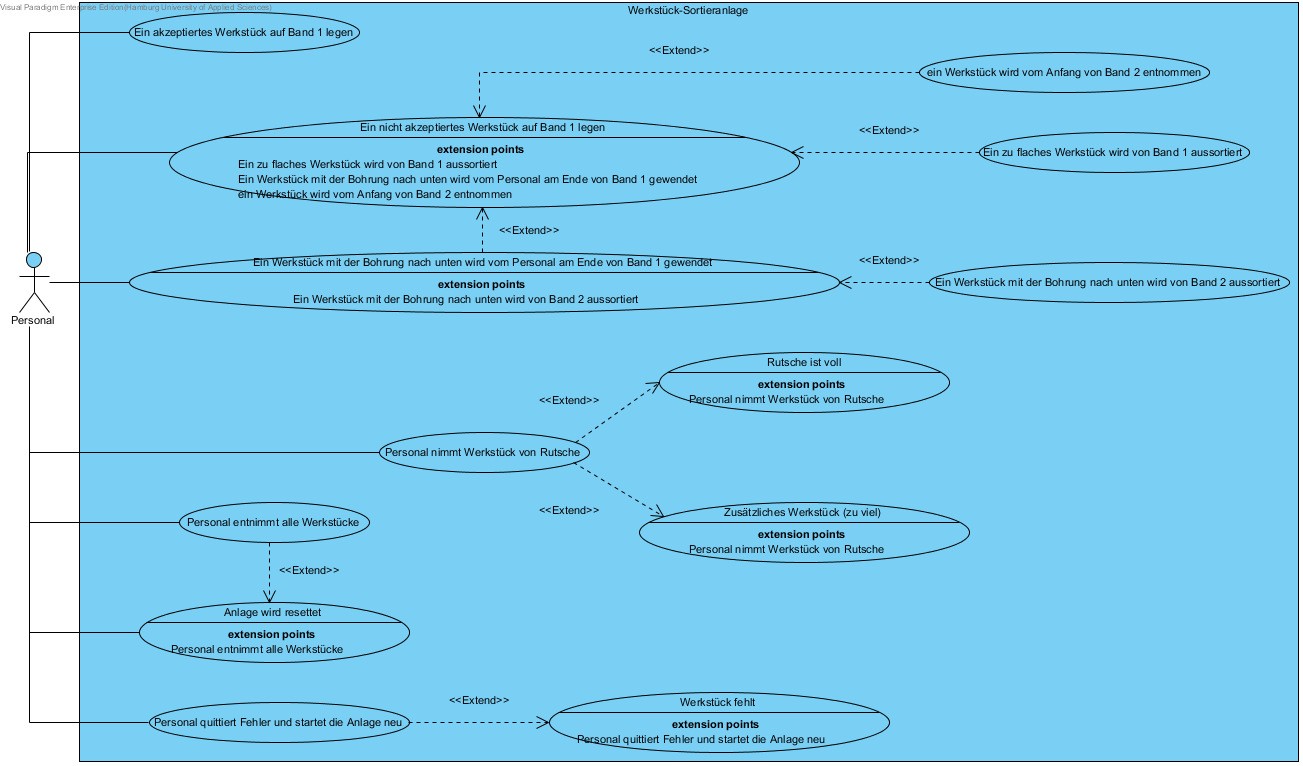
\includegraphics[angle=90,scale=0.7]{imgs/UseCases.png}
  \caption{Use-Case-Diagramm}
\end{figure}

% 5.5 Systemanalyse
\subsection{Systemanalyse}
Das System wird über ein C++-Programm gesteuert, welches auf einem bzw. zwei (bei Nutzung von zwei Förderbändern) GEME-Rechnern läuft. Die Aktorik und Sensorik werden über 3 Ports angesteuert, wobei die Sensoren die Werte mittels Interrupts dem System mitteilen.\newline
Die Kommunikation der beiden Förderbänder läuft über eine serielle Schnittstelle. Es werden hier z.B. die Messergebnisse von Band 1 an Band 2 übergeben, damit, wenn ein Puck das Ende von Band 2 erreicht, seine zugehörigen Daten ausgegeben werden können. Nachrichteneingänge über die serielle Schnittstelle werden ebenfalls durch Interrupts realisiert.

\newpage

% 6. Design
\section{Design}

% 6.1 System-Architektur
\subsection{System-Architektur}
Das System verfügt über folgende Module: HAL zum Ansteuern/Auslesen der Aktorik und Sensorik, seriellen Bus zur Ansteuerung der seriellen Schnittstelle, FSM zur Anlagensteuerun, Dispatcher, der die Pulse Messages entgegennimmt, Timer zur Zeitmessung/-kontrolle und util(mutex, condvar, lockguard, logging, singleton\_mgr, HAWThread, light\_mgr). Des Weiteren gibt es zugehörige Unit-Tests.

% 6.1.1 Komponenten-Diagramm
\begin{figure}[h]
  \subsubsection{Komponenten-Diagramm}
  \centering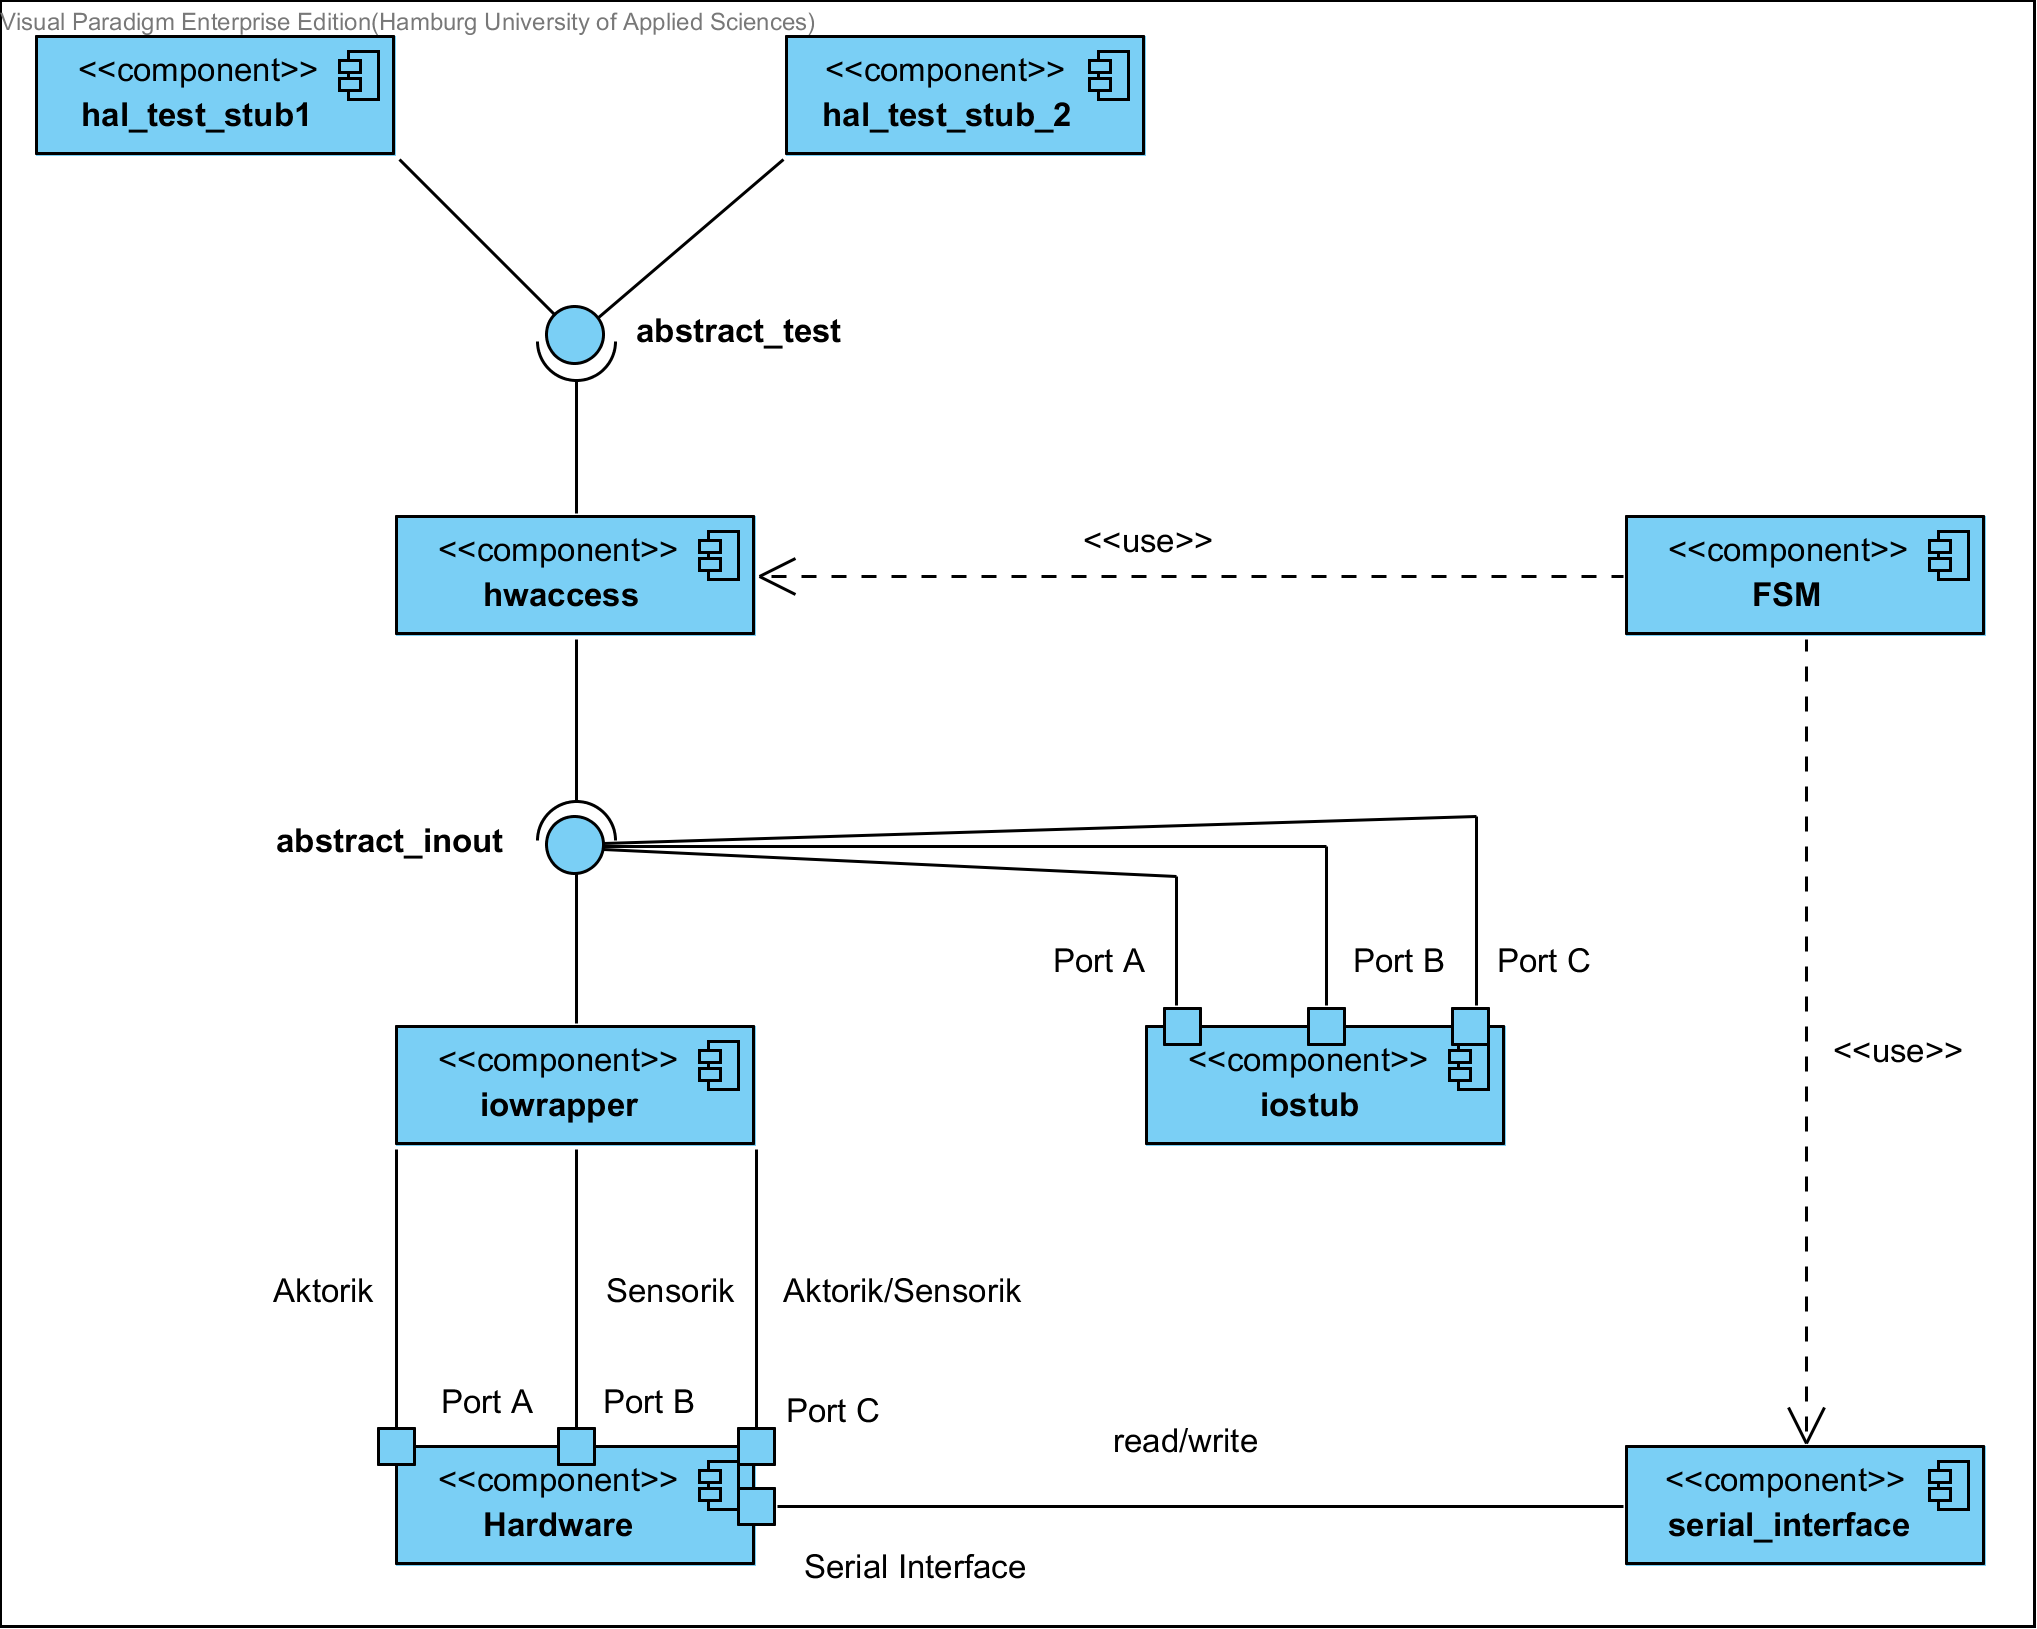
\includegraphics[angle=0,scale=0.93]{imgs/Sortieranlage-Komponenten.png}
  \caption{Komponenten-Diagramm}
\end{figure}

% 6.2 Datenmodell
\subsection{Datenmodell}
siehe Klassendiagramm im imgs-Ordner

% 6.3 Datenmodell
\subsection{Verhaltensmodell}
siehe Abbildungen 3-5 auf den Seiten 19-21

% 6.3.1 Automat für Band 1
\begin{figure}[p]
  \subsubsection{Automat für Band 1}
  \centering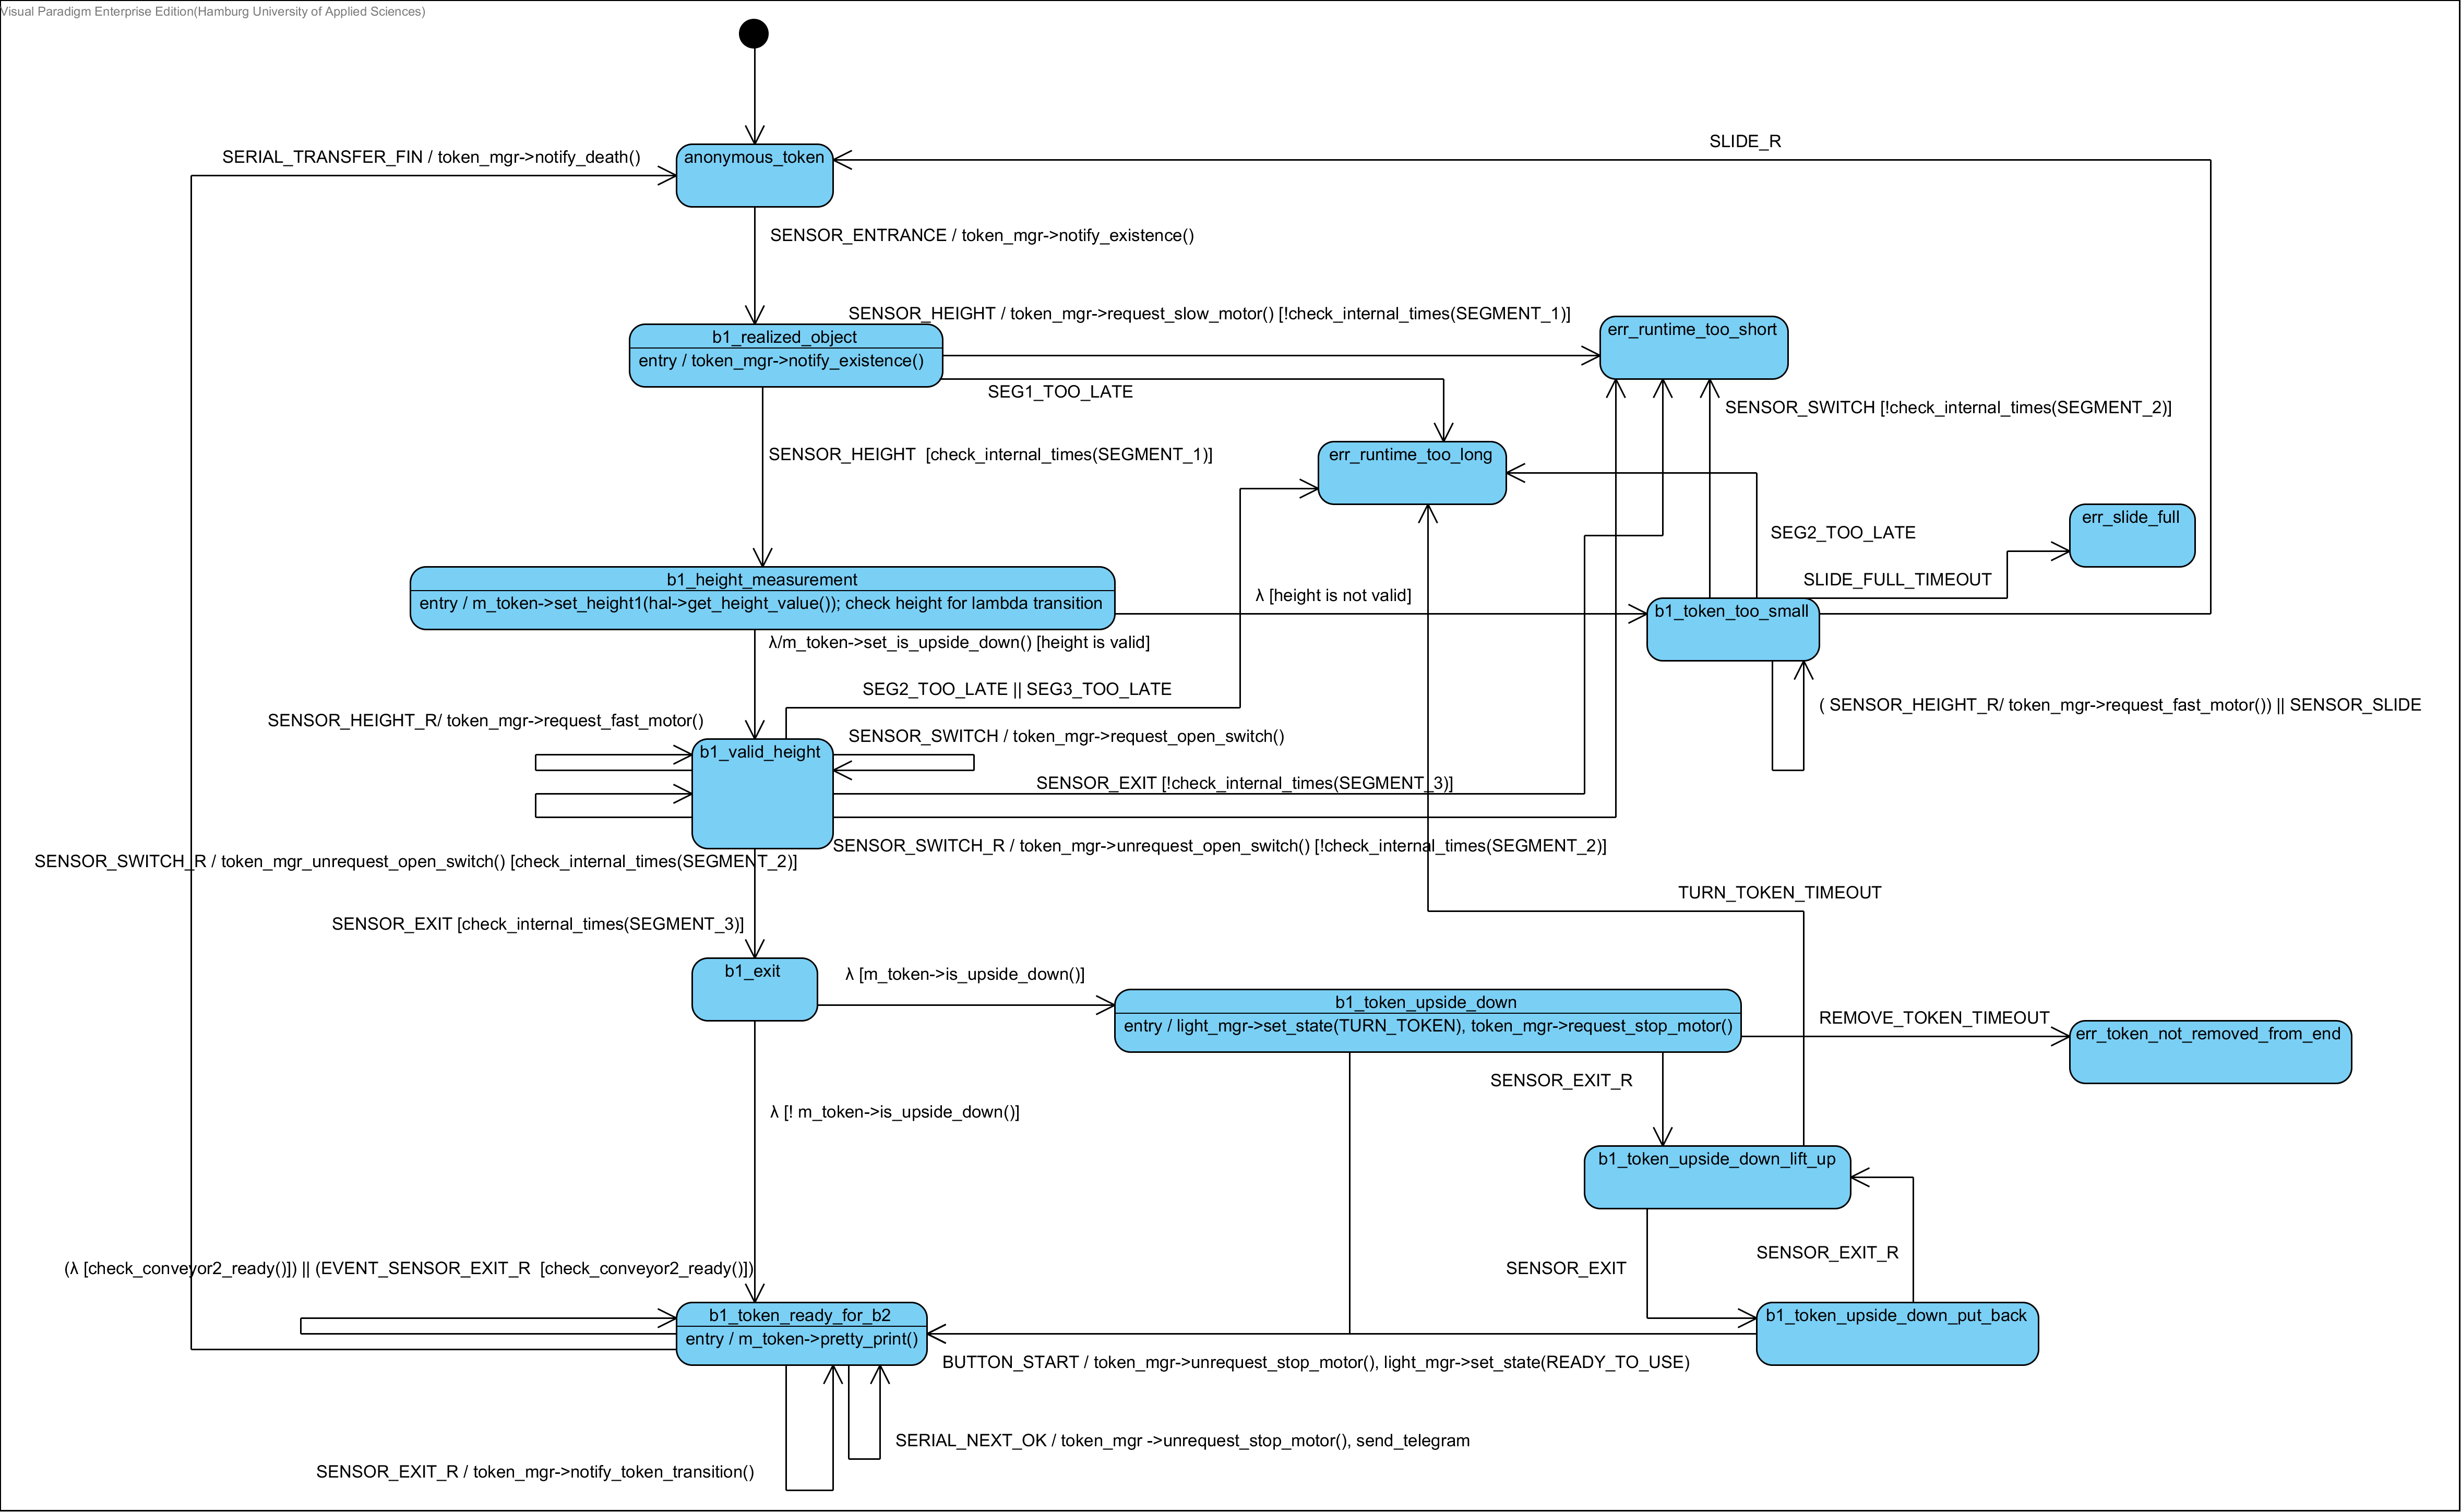
\includegraphics[angle=90,scale=0.59]{imgs/Band1_FSM.png}
  \caption{Automat für Band 1}
\end{figure}

% 6.3.2 Automat für Band 2
\begin{figure}[p]
  \subsubsection{Automat für Band 2}
  \centering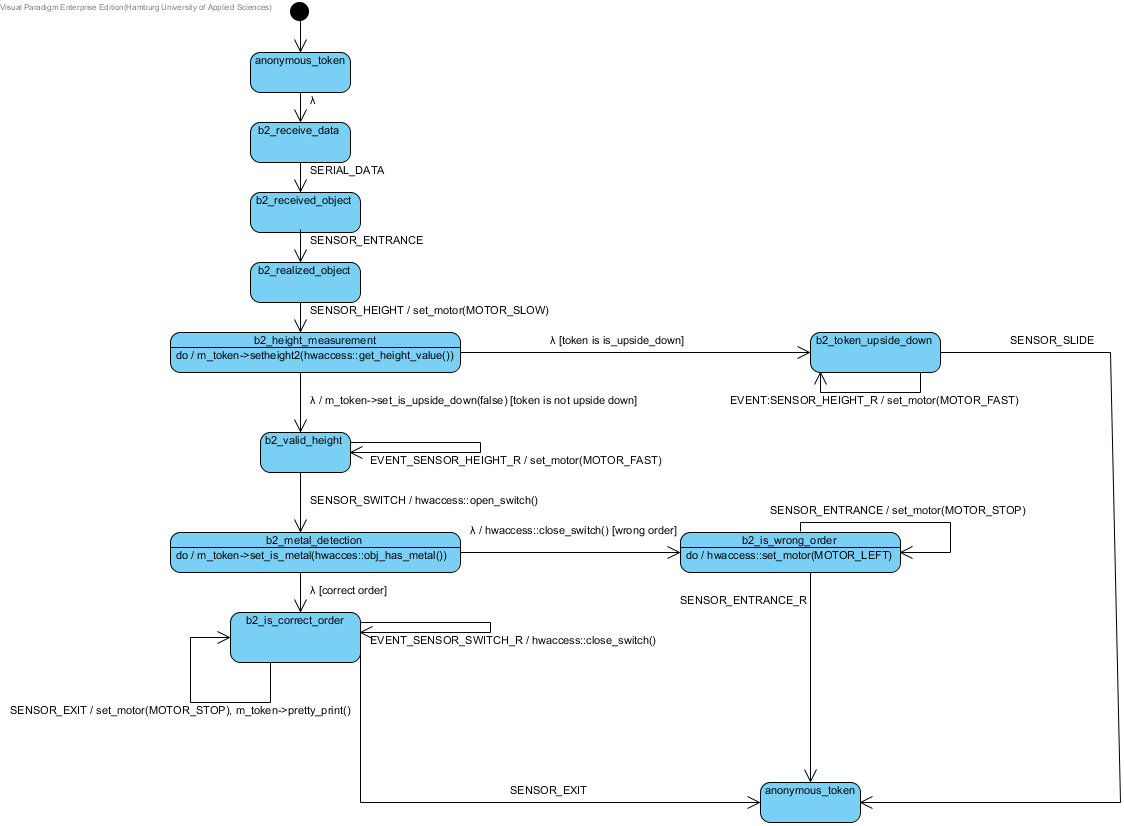
\includegraphics[angle=90,scale=0.635]{imgs/Band2_FSM.png}
  \caption{Automat für Band 2}
  \clearpage
\end{figure}

% 6.3.3 Automat für die Fehlerbehebung
\begin{figure}[p]
  \subsubsection{Automat für die Fehlerbehebung}
  \centering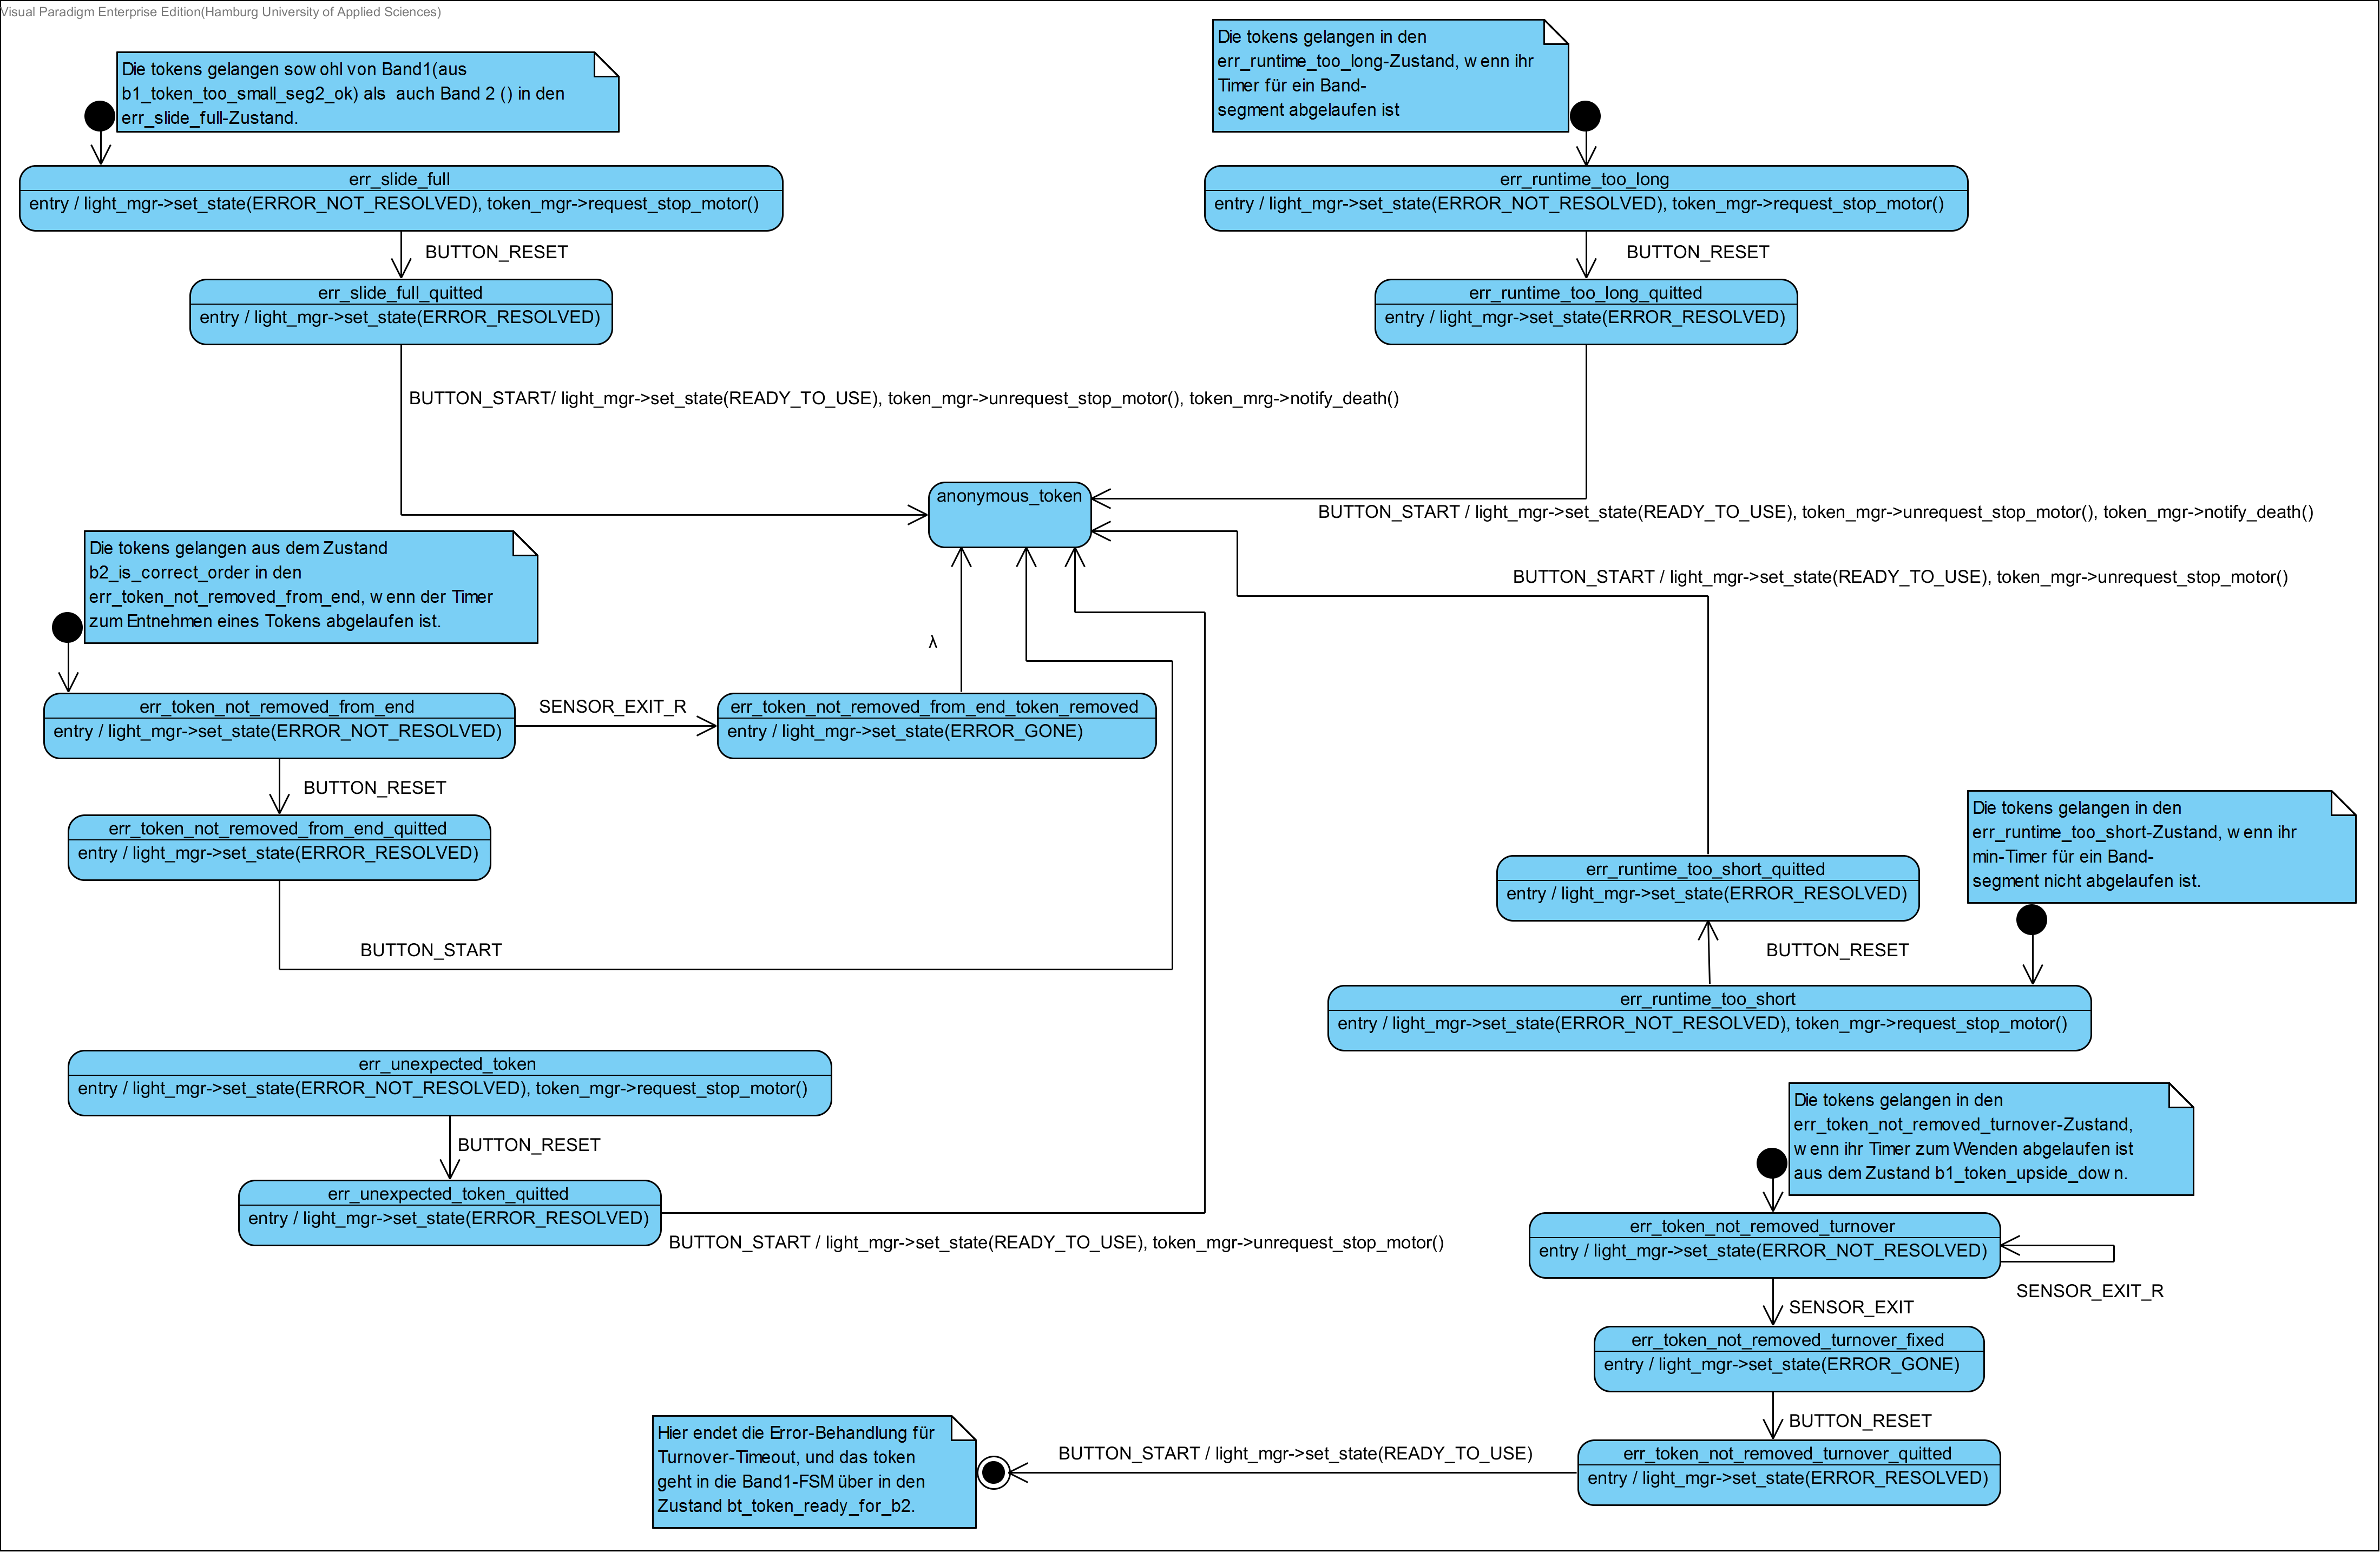
\includegraphics[angle=90,scale=0.63]{imgs/Error_FSM.png}
  \caption{Automat für die Fehlerbehebung}
\end{figure}


% 7. Implementierung
\section{Implementierung}

% 7.1 Patterns
\subsection{Patterns}
Scoped Locking, DCLP, Singelton, Delegator, Factory, Dispatcher-/Reactor-Pattern und GoF-State-Pattern nach Pareigis.

% 7.2 Interrupt Implementierung
\subsection{Interrupt-Implementierung}
Die ISR soll eine Pulse Message generieren. Diese landet im Pulse Message Channel, der vom Dispatcher abgehört wird.
Der Code in der Pulse Message spezifiziert die Quelle des Ereignisses. Als zusätzlicher Integer wird das geänderte Bit angehängt. Dabei wird Port A um 8 Bits nach links geschoben. Port B wird per Veroderung angehängt. Als Vergleich dienen die Port-Werte vor dem Interrupt. Um nun das geänderte Bit zu erkennen, werden aktueller Wert und alter Wert per Exklusiv-Oder verknüpft.

% 7.3 Dispatcher Implementierung
\subsection{Dispatcher-Implementierung}
Die Implementierung des Dispatchers verteilt Events (Eingangsereignisse) an angemeldete Zustände.
Als Quellen für Eingangssignale dienen ISR, Timer, Serielle Schnittstelle. Intern werden die Signale
nur an den ersten Zustand einer FIFO weitergereicht. Für jeden anmeldbaren Zustand gibt es eine eigene FIFO.\newline
Als FIFO Container wurde die std::queue benutzt. Jede Queue geht über Pointer-to-Memberfunktionen.
Im System existiert ein Pulse Message-Channel, in den die Eingangssignalquellen Pulse Messages schreiben.
Der Dispatcher implementiert einen eigenen Thread, der diese Pulse Messages aus dem Channel liest und die passende Pointer-to-Memberfunktion aufruft.

% 7.4 Automaten Implementierung
\subsection{Automaten-Implementierung}
Die Automaten werden nach dem GoF-State-Pattern nach Pareigis umgesetzt. Die Transition findet durch den
Placement-New Operator statt. Die Kontext-Klasse \emph{token} dient der Abbildung eines Pucks. In ihr werden die
Eigenschaften des Pucks und dessen Zustand gespeichert.\newline
Die Zustände des Pucks werden durch die Klasse \emph{state} repräsentiert. Sie leitet sich von der Klasse
\emph{events} ab, die die Transitionen in Form von \emph{pure virtual} Funktionen vorgibt.\newline
Jeder Subzustand von \emph{state} meldet sich für ein Event beim Dispatcher an und implementiert die Transition
für diesen.\newline
Der Start- und Endzustand eines jeden Tokens ist \emph{anonymous\_token}.\newline
Der Dispatcher führt eine Queue über die Anzahl der maximal auf einem Band befindlichen Tokens, die mit dem Zustand
\emph{anonymous\_token} vorinitialisiert werden.

\newpage

% 7.5 Timer Implementierung
\subsection{Timer Implementierung}
Die QNX eigenen Timer-Funktionen werden in \emph{timer\_wrapper} gewrapped, um von dem \emph{timer\_handler} verwaltet zu werden. Bei diesem \emph{timer\_handler} können Timer mit einer Zeitspanne registriert werden.
Die registrierten Timer können pausiert, fortgesetzt, addiert, subtrahiert und gestoppt werden.\newline\newline
Timer werden eingesetzt:
\begin{itemize}
    \item Um zu prüfen, ob Werkstücke hinzugefügt oder entfernt wurden
    \item Um zu prüfen, ob die Rutsche voll ist
    \item Um die Ampel blinken zu lassen
\end{itemize}

% 7.5.1 Diskussion der Hardware- und Betriebssystem-Timer
\subsubsection{Diskussion der Hardware- und Betriebssystem-Timer}
QNX stellt 3 Arten von Timern zu Verfügung:

\begin{itemize}
  \item Realtime
  \item Monotonic
  \item Softtime
\end{itemize}
Der Realtime-Timer lässt sich durch Zeitänderung ein wenig manipulieren. Der Timer wird aktiv, sobald der Zeitpunkt: Timer-Zeit plus Startzeitpunkt erreicht wurde.
Wenn z.B. die BS Zeit sich während des Timers synchronisiert und dadurch um einen Augenblick erhöht, so schlägt der Realtime-Timer trotzdem an dem errechneten Zeitpunkt an, auch wenn die Zeit in Wirklichkeit noch nicht verstrichen ist.\newline
Der Monotonic-Timer hingegen lässt sich nicht von diesen Zeiten beeinflussen. Er zählt seine Takte und wenn diese erreicht wurden, wird er aktiv.\newline
Ein Softtime-Timer ist nur aktiv, wenn auch die CPU läuft. Dieser Timer kann die CPU nicht wecken und schlägt erst Alarm, wenn er wieder aktiv ist.

\newpage

% 8. Testen
\section{Testen}

% 8.0 Testplan
\subsection{Testplan}
Da nach dem V-Modell vorgegangen wird, wird zu jedem Milestone die Funktionalität der für den Milestone benötigten Punkte getestet.

% 8.1 Unit-Test/Komponenten-Test
\subsection{Unit-Test/Komponenten-Test}
Es gibt Testfälle für die einzelnen Komponenten. Für die Unit-Tests steht eine Testumgebung zur Verfügung.
Jeder Unit-Test muss das Abstract-Test-Interface implementieren, damit diese automatisiert ausgeführt werden
können.

% 8.1.1 HAL
\subsubsection{HAL}
Im Unit Test für die HAL werden zwei verschiedene Stubs verwendet. Die Hardware wird dafür nicht verwendet,
da diese Stubs das Verhalten der Hardware emulieren. Alle Funktionen der HAL werden bei dem Test einmal durchlaufen
und es wird geprüft, ob die Funktionen die erwarteten Rückgabewerte liefern.

% 8.1.2 IRQ
\subsubsection{IRQ}
Der automatisierte IRQ/ISR Test öffnet einmal die Weiche. Dabei wird die Lichtschranke der Weiche unterbrochen,
was eine Pulse Message generiert. Diese muss im Channel liegen.

% 8.1.3 Dispatcher
\subsubsection{Dispatcher}
Für den Dispatcher gibt es verschiedene Unit-Tests. Zum einen wird getestet,
ob das Mapping vom Event-enum zum internen Dispatched-Event-enum passt.
Zum anderen wird geprüft, ob in dem Funktionsadressen-Array die korrekten Adressen liegen.\newline
Ein weiterer Test prüft, ob der Dispatcher die Events sequenziell verteilt. Dazu gibt es eine
FSM, die nur aus einem Zustand besteht, jedoch für jede Eingabe eine Transition auf sich selbst hat.\newline
Bei der Transition wird geprüft, ob das erhaltene Eingangssignal das erwartete Eingangssignal ist.
Die FSM wird zweimal durchlaufen. Beim ersten Mal wird der Dispatcher-Thread umgangen, indem die Events
direkt aufgerufen werden. Das zweite Mal schreibt Pulse Messages in den Channel, die vom Dispatcher
verteilt werden.

% 8.1.4 Timer
\subsubsection{Timer}
Beim Timer werden die Grundfunktionalitäten getestet.\newline
Zum Testen der Registrierungsfunktion wird ein Timer gestartet und auf die Pulse Message gewartet.\newline
Um die Funktionen add, sub, pause und continue zu testen, wird jedoch ein weiterer Timer registriert.
Dieser zusätzliche Timer sendet eine andere Message beim Ablaufen, wodurch verhindert wird, dass kein Interrupt
geworfen wird.

\newpage

% 8.2 Integrations-Test/System-Test
\subsection{Integrations-Test/System-Test}
\textbf{Beim Systemtest werden folgende Szenarien getestet:}
\begin{enumerate}
  \item Es werden zu flache Pucks auf Band 1 gelegt, um zu prüfen, ob diese von Band 1 aussortiert werden.
  \item Es werden mehrere Werkstücke gleichzeitig auf Band 1 gelegt. Dabei wird überprüft, ob Band 1 stoppt und mit der Übergabe der Pucks wartet, bis Band 2 frei ist.
  \item Es werden Werkstücke in richtiger und falscher Reihenfolge auf Band 1 gelegt. Dabei wird überprüft, ob Band 2 ein betreffendes Puck zurück an den Anfang fährt und auf dessen Entnahme wartet, um die richtige Reihenfolge wiederherzustellen.
  \item Es werden Werkstücke mit der Bohrung nach unten auf Band 1 gelegt. Dabei wird überprüft, ob Band 1 stoppt, damit das Personal den Puck wenden kann, und bei Zurücklegen des Pucks weiterfährt, sofern Band 2 frei ist.
  \item Es werden Werkstücke mit der Bohrung nach unten auf Band 1 gelegt, die nicht vom Personal gewendet werden, um zu prüfen, ob diese Pucks von Band 2 aussortiert werden.
  \item Es werden Pucks im laufenden Betrieb an allen Segmenten entnommen oder hinzugefügt, um zu prüfen, ob die Zeitüberwachung dieser Segmente richtig arbeitet.
  \item Es werden zu flache Pucks auf Band 1 gelegt, bis die Rutsche voll ist, um zu prüfen, ob dessen Fehlerabarbeitung von Band 1 richtig arbeitet.
  \item Pucks mit der Bohrung nach unten werden am Ende von Band 2 nicht gewendet, bis die Rutsche von Band 2 voll ist, um zu prüfen, ob dessen Fehlerbearbeitung von Band 2 richtig arbeitet.
\end{enumerate}

\newpage

% 8.4 Regressions-Test
\subsection{Regressions-Test}
Die wichtigsten Hauptkomponenten haben jeweils eigene Regressions-Tests. Diese sind möglichst unabhängig voneinander und werden zur Qualitätssicherung durchgeführt.
\begin{enumerate}
  \item \textbf{Test der HAL}
  \begin{enumerate}
    \item Alle HAL Funktionalitäten werden auf ihre positiven Fälle geprüft. (Benötigt keine Hardware, da durch Stubs realisiert)
    \item Alle HAL Funktionalitäten werden einmal auf ihr invertiertes Verhalten geprüft. (Benötigt keine Hardware, da durch Stubs realisiert)
  \end{enumerate}
  \item \textbf{Test der ISR/IRQ}
  \begin{enumerate}
    \item Die Weiche wird per HAL geöffnet. Die Lichtschranke der Weiche durchbrochen, dadurch wird die ISR ausgeführt und eine Pulse Message generiert. Diese wird ausgewertet.
  \end{enumerate}
  \item \textbf{Test des Dispatchers}
  \begin{enumerate}
    \item Es wird geprüft ob das Enum-Mapping vom externen Typ \emph{event\_values} zum internen Typ \emph{dispatcher\_events} korrekt funktioniert.
    \item Es wird geprüft ob im Funktionspointerarray des Dispatchers die korrekten Adressen stehen.
    \item Die Dispatcher interne Funktion zum ausführen der Funktionspointer wird geprüft, dazu wird jedes Event einmal direkt mit der Funktion aufgerufen.
    \item Der Dispatcher selbst wird geprüft indem jede gültige Pulse Message in den Channel des Dispatchers geschrieben wird, die korrekte Reihenfolge der Abarbeitung wird hierbei geprüft.
  \end{enumerate}
  \item \textbf{Test der Timer}
  \begin{enumerate}
    \item Ein normaler Timer wird erstellt, dieser soll nach einer Millisekunde einen Wert in einen Pulse Message Channel schreiben. Der Wert der Pulse Message wird geprüft.
    \item Ein Timer mit kurzer Laufzeit und ein zweiter Timer mit längerer Laufzeit wird erstellt. Der erste Timer wird pausiert. Es wird blockiert bis eine Pulse Message vorhanden ist. Danach wird der kurze Timer fortgesetzt und auf die Pulse Message gewartet.
    \item Es werden drei Timer erstellt. Einer mit 500 Millisekunden Laufzeit, einer mit einer Sekunde Laufzeit, sowie einer mit drei Sekunden. Nachdem alle gestartet sind, wird dem 500 Millisekunden Timer eine Sekunde hinzugefügt. Die korrekte Reihenfolge der Pulse Messages wird ausgewertet.
  \end{enumerate}
  \item \textbf{Test der Seriellen Schnittstelle}
  \begin{enumerate}
    \item Senden/Empfangen eines Daten-Telegramms
    \item Auswerten der Daten (Prüfung ob Daten korrekt empfangen wurden)
    \item Senden/Empfangen im Full-Duplex-Betrieb
  \end{enumerate}
\end{enumerate}
\textbf{Die Regressions-Tests wurden in den Unit-Tests umgesetzt.}

\newpage

% 8.5 Abnahme-Test
\subsection{Abnahme-Test}
Um eine komplette Abdeckung der zu Beginn des Projekts aufgestellten Requirements zu gewährleisten, wurden Abnahme-Tests entworfen.\newline
Die Auflistung dieser Tests findet sich in den Unterpunkten 8.5.1 und 8.5.2.\newline
Eine Übersicht, welcher Abnahme-Test welche Requirements abdeckt, findet sich in den darauffolgenden Abbildungen der Unterpunkte 8.5.3 - 8.5.5.

% 8.5.1 Abnahme-Tests für die Grundfunktionen der Anlage
\subsubsection{Abnahme-Tests für die Grundfunktionen der Anlage}
\textbf{Mindestabstand: 5cm}
% Tabelle
\begin{small}
  \begin{center}
    \begin{longtable}{|c|p{4cm}|p{6cm}|C{3cm}|}
      \hline
      \textbf{Test-ID} & \textbf{Beschreibung} & \textbf{Erwartung} & \textbf{Requirement-ID}\\
      \toprule
      \endhead
      \hline
      TG00 & Hardware-Check & Es gibt zwei hintereinander gestellte, richtig angeschlossene
      und funktionsfähige Förderbänder, auf die nur die definierten Pucks gelegt werden.
      Beide Förderbänder besitzen jeweils eine Ampelanlage. & FR-001, FR-002, FR-016, FR-019.1, FR-024.1, FR-024.2, FR-027, FR-028, FR-029.1, FR-030.1, FR-030.2\\
      \hline
      \rowcolor{lightgray} TG01 & Es wird ein zu kleiner Puck auf B1 gelegt. & Der Puck fährt langsam durch die Höhenmessung und wird auf B1 aussortiert. & FR-004, FR-006.1, FR-006.2, FR-014, FR-019.5\\
      \hline
      TG02 & Es werden Pucks mit dem Mindestabstand von 5cm in der Reihenfolge Metall, Nicht-Metall, Metall auf B1 gelegt. Sobald ein Puck das Ende von B2 erreicht, wird dieser entfernt. & Der erste Puck (Metall) fährt bis ans Ende von B2, gibt auf der Konsole die Daten (ID, Höhenmesswert von B1, Höhenmesswert von B2, Typ) aus und wartet.
      Die B2-Ampel blinkt orange, bis dieser Puck entfernt wird.
      Der zweite Puck (Nicht-Metall) fährt bis ans Ende von B1 und wartet, bis der erste von B2 entfernt wird.
      Sobald der erste Puck entfernt wird, fährt der zweite ans Ende von B2 und gibt dann seine Daten aus.
      Der dritte Puck verhält sich wie der Zweite. Er hält am Ende von B1 und fährt auf B2, sobald dieses wieder frei ist. Während der gesamten Zeit leuchtet die Ampel auf B1 grün.
      Wenn der dritte Puck auf B2 ist, hält B1 an und auch wenn er von B2 entnommen wird fährt keines der beiden wieder los. & FR-003.1, FR-003.2, FR-004, FR-005, FR-008.1, FR-009.1, FR-009.3, FR-009.4, FR-010, FR-011, FR-012.1, FR-012.2, FR-013, FR-014, FR-015, FR-017, FR-018.2, FR-020, FR-026, NFR-003, NFR-004.1, NFR-005\\
      \hline
      \rowcolor{lightgray} TG03 & Ein Nicht-Metall-Puck wird mit der Bohrung nach unten auf B1 gelegt. Am Ende von B1 wird der Puck gewendet und die Start-Taste wird betätigt. & Der Puck fährt bis ans Ende von B1. B1 hält an und die Ampel blinkt orange. Erst nach Betätigen der Start-Taste erlischt das orange Blinken und der Nicht-Metall-Puck fährt an das Ende von B2. & FR-004, FR-007.1, FR-007.2, FR-007.3, FR-007.4, FR-007.5, FR-009.4, FR-014, FR-015, FR-018.1, FR-019.5, FR-026, NFR-001, NFR-003, NFR-004.1\\
      \hline
      TG04 & Ein Metall-Puck und ein verkehrt herum liegender Nicht-Metall-Puck werden mit dem Mindestabstand von 5cm auf B1 gelegt. Der erste richtig herum liegende Puck wird entnommen, sobald der zweite Puck das Ende von B1 erreicht hat. Der verkehrt herum liegende Puck wird nicht gewendet und die Start-Taste auf B1 wird betätigt. & Der Metall-Puck fährt bis ans Ende von B2. B1 hält an, sobald der verkehrt herum liegende Puck das Ende erreicht, und die orange Ampel blinkt. B1 fährt nicht los, auch wenn der erste Puck von B2 entfernt wird.
      Die Starttaste von B1 wird ohne Wenden des Pucks betätigt, sodass der verkehrt herum liegende Puck auf B2 aussortiert wird. & FR-003.2, FR-004, FR-005, FR-007.1, FR-007.2, FR-007.3, FR-007.4, FR-008.1, FR-008.2, FR-009.3, FR-009.4, FR-010, FR-011, FR-012.1, FR-012.2, FR-013, FR-014, FR-015, FR-018.1, FR-018.2, FR-019.5, FR-026, NFR-003, NFR-004.1, NFR-005\\
      \hline
      \rowcolor{lightgray} TG05 & Zwei Pucks ohne Metall werden mit dem festgelegten Mindestabstand von 5cm auf B1 gelegt. Die Pucks werden entnommen, sobald die Ampel von B2 orange blinkt.
       & Der erste Puck fährt bis ans Ende von B2. Der zweite Puck fährt auf B2, sobald der erste entfernt wurde, jedoch nur bis zum Metallsensor. Dann wird er wieder an den Anfang von B2 zurück befördert. Sobald der Puck den Anfang von B2 erreicht, hält dieses an und die Ampel von B2 blinkt orange, bis der Puck entfernt wird. & FR-003.2, FR-004, FR-005, FR-009.1, FR-009.2, FR-009.3, FR-009.4, FR-010, FR-011, FR-012.1, FR-012.2, FR-013, FR-014, FR-015, FR-017, FR-018.2, FR-019.5, FR-020, NFR-003, NFR-004.1, NFR-005\\
      \hline
      TG06 & Zwei Pucks mit Metall werden mit dem Mindestabstand von 5cm auf B1 gelegt. Die Pucks werden entnommen, sobald die Ampel von B2 orange blinkt. & Der erste Puck fährt bis ans Ende von B2. Der zweite Puck fährt auf B2, sobald der erste entfernt wurde, jedoch nur bis zum Metallsensor und wird dann wieder an den Anfang von B2 befördert. Dort hält er an und die Ampel von B2 blinkt orange, bis der Puck entfernt wird. & FR-003.2, FR-004, FR-005, FR-009.1, FR-009.2, FR-009.3, FR-009.4, FR-010, FR-011, FR-012.1, FR-012.2, FR-013, FR-014, FR-015, FR-017, FR-018.2, FR-019.5, FR-020, NFR-003, NFR-004.1, NFR-005\\
      \hline
    \end{longtable}
  \end{center}
\end{small}

\newpage

% 8.5.2 Abnahme-Tests für die Fehlerfälle der Anlage
\subsubsection{Abnahme-Tests für die Fehlerfälle der Anlage}
\textbf{Mindestabstand: 5cm}
% Tabelle
\begin{small}
  \begin{center}
    \begin{longtable}{|c|p{4cm}|p{6cm}|C{3cm}|}
      \hline
      \textbf{Test-ID} & \textbf{Beschreibung} & \textbf{Erwartung} & \textbf{Requirement-ID}\\
      \toprule
      \endhead
      \hline
      TF01 & Ein Metall-Puck und ein Nicht-Metall-Puck mit Bohrung nach unten werden mit dem Mindestabstand von 5cm auf B1 gelegt. Der erste Puck wird entnommen, wenn er am Ende von B2 ist und sobald der zweite Puck das Ende von B1 erreicht hat. Der verkehrt herum liegende Puck wird nur hochgenommen, aber nicht gewendet, und die Start-Taste von B1 wird betätigt. & Der zweite Puck fährt bis ans Ende von B1. Dieses hält an und die Ampel von B1 blinkt orange. Das orange Blinken wechselt nach ca. 15 Sekunden in ein rotes Blinken. Sobald der Fehler quittiert wird, wechselt das rote Blinken in ein Dauerlicht. Sobald der Puck entfernt, der Fehler quittiert und die Start-Taste betätigt wird, geht das Band wieder in den betriebsbereiten Zustand und die Ampel von B1 leuchtet grün. & FR-004, FR-007.1, FR-007.2, FR-007.3, FR-007.4, FR-007.5, FR-013, FR-014, FR-017, FR-018.1, FR-019.2, FR-019.3, FR-029.2\\
      \hline
      \rowcolor{lightgray} TF02 & Ein Nicht-Metall-Puck wird auf B1 gelegt. Der Puck wird auf B2 vor der Höhenmessung entfernt. & Das Band hält an und die Ampel von B2 blinkt rot. & FR-004, FR-010, FR-011, FR-016, FR-019.1, FR-019.2, FR-019.3, FR-019.5, FR-021, FR-025, FR-029.1, FR-029.2, NFR-004.1, NFR-004.3\\
      \hline
      TF03 & Ein Metall- und ein Nicht-Metall-Puck werden mit dem Mindestabstand von 5cm auf B1 gelegt. Zwischen Höhenmessung und Weiche wird der Metall-Puck von dem Band entfernt. & Das Band hält an und die Ampel von B1 blinkt rot. & FR-004, FR-010, FR-011, FR-016, FR-019.1, FR-019.2, FR-019.3, FR-019.5, FR-021, FR-025, FR-029.1, FR-029.2, NFR-004.1, NFR-004.3\\
      \hline
      \rowcolor{lightgray} TF04 & Es werden Nicht-Metall-, Metall-, Nicht-Metall-Pucks auf B1 gelegt. Nach der Weiche wird der Metall-Puck (Zweite) von B1 entfernt. Der Fehler wird quittiert und die Bänder neu gestartet. Danach wird ein Metall-Puck auf B1 gelegt. & Das Band hält an und die Ampel von B1 blinkt rot. Nach dem Quittieren und Starten leuchtet die Ampel wieder grün und das Band ist betriebsbereit. Der neue Metall-Puck wird wieder befördert. & FR-004, FR-010, FR-011, FR-016, FR-019.1, FR-019.2, FR-019.3, FR-019.5, FR-021, FR-025, FR-029.1, FR-029.2, NFR-004.1, NFR-004.3\\
      \hline
      TF05 & Manuell werden drei zu kleine Pucks in die Rutsche von B1 gelegt. Danach wird ein zu kleiner Puck an den Anfang von B1 gelegt. Nach Auftreten des Fehlers wird ein Puck aus der Rutsche genommen. & Der zu kleine Puck wird auf B1 aussortiert. Es wird erkannt, dass die Rutsche voll ist. B1 geht in den Fehlerzustand über, die Ampel blinkt schnell rot. Wenn der Puck entfernt wird, wechselt das schnelle Blinken in ein langsames. & FR-004, FR-006.1, FR-006.2, FR-011, FR-016, FR-017, FR-019.1, FR-019.2, FR-019.3, FR-019.4, FR-019.5, FR-023\\
      \hline
      \rowcolor{lightgray} TF06 & Zwei Nicht-Metall-Pucks werden so auf B1 gelegt, dass ein weiterer Puck dazwischen passt. Vor der Höhenmessung wird ein Metall-Puck dazwischen gelegt. & Das Band hält an und die Ampel von B1 blinkt rot. & FR-009.1, FR-009.2, FR-009.3, FR-009.4, FR-011, FR-016, FR-017, FR-019.1, FR-019.2, FR-019.3, FR-019.5, FR-029.1, FR-029.2, NFR-004.1, NFR-004.2\\
      \hline
      TF07 & Ein Metall-Puck wird auf B1 gelegt. Sobald der Puck in der Höhenmessung auf B2 ist, wird ein Nicht-Metall-Puck vor den Metallsensor auf B2 gelegt. & Das Band hält an und die Ampel von B2 blinkt rot. & FR-004, FR-012.2, FR-016, FR-017, FR-019.1, FR-019.2, FR-019.3, FR-019.5, FR-022, FR-029.1, FR-029.2, NFR-004.1, NFR-004.2\\
      \hline
      \rowcolor{lightgray} TF08 & Ein Nicht-Metall-Puck wird auf B1 gelegt. Während der Puck noch vor der Weiche ist, wird ein Metall-Puck hinter die Weiche gelegt. & Das Band hält an und die Ampel von B1 blinkt rot. & FR-004, FR-011, FR-017, FR-019.1, FR-019.2, FR-019.3, FR-019.5, FR-022, FR-029.1, FR-029.2, NFR-004.1, NFR-004.2\\
      \hline
      TF09 & Ein Metall-Puck wird auf B1 gelegt. Wenn dieser Puck am Ende von B2 ankommt, wird er nicht entnommen, sodass das Band in den Fehlerzustand übergeht. Dann wird der Puck entnommen und ein weiterer Metall-Puck wird an den Anfang von B1 gelegt. & Der erste Puck fährt bis ans Ende von B2 und löst den Fehlerzustand aus. Wenn der Puck von B2 entfernt wird und ein neuer Puck auf B1 liegt, darf dieser nur bis ans Ende von B1 fahren, aber nicht weiter, da B2 noch im Fehlerzustand ist. & FR-004, FR-005.1, FR-005.2, FR-015.2, FR-017, FR-018.2, FR-019.1, FR-019.2, FR-019.3, FR-019.5, FR-029.1, NFR-003\\
      \hline
      \rowcolor{lightgray} TF10 & Ein Metall-Puck wird auf B1 gelegt. Sobald der Puck auf B2 ist, wird ein weiterer Metall-Puck auf B1 gelegt. Anschließend wird die E-Stopp-Taste von B2 gedrückt. & Beide Bänder gehen in den Safe-State und die Programme beenden sich. & FR-004, FR-012.1, FR-017, FR-030.1, FR-030.2, FR-030.3\\
      \hline
      TF11 & Ein Metall-Puck wird mit der Bohrung nach unten auf B1 gelegt. Am Ende von B1 wird dieser entnommen. & Etwa 15 Sekunden nachdem der Puck entnommen wurde, geht das Band in den Fehlerzustand. & FR-004, FR-007.1, FR-007.2, FR-007.3, FR-007.4, FR-007.6, FR-013, FR-014, FR-015.1, FR-016, FR-017, FR-018.1, FR-019-2\\
      \hline
    \end{longtable}
  \end{center}
\end{small}

% 8.5.3 Abdeckung der Functional Requirements [1/2]
\begin{figure}[p]
  \subsubsection{Abdeckung der Functional Requirements [1/2]}
  \centering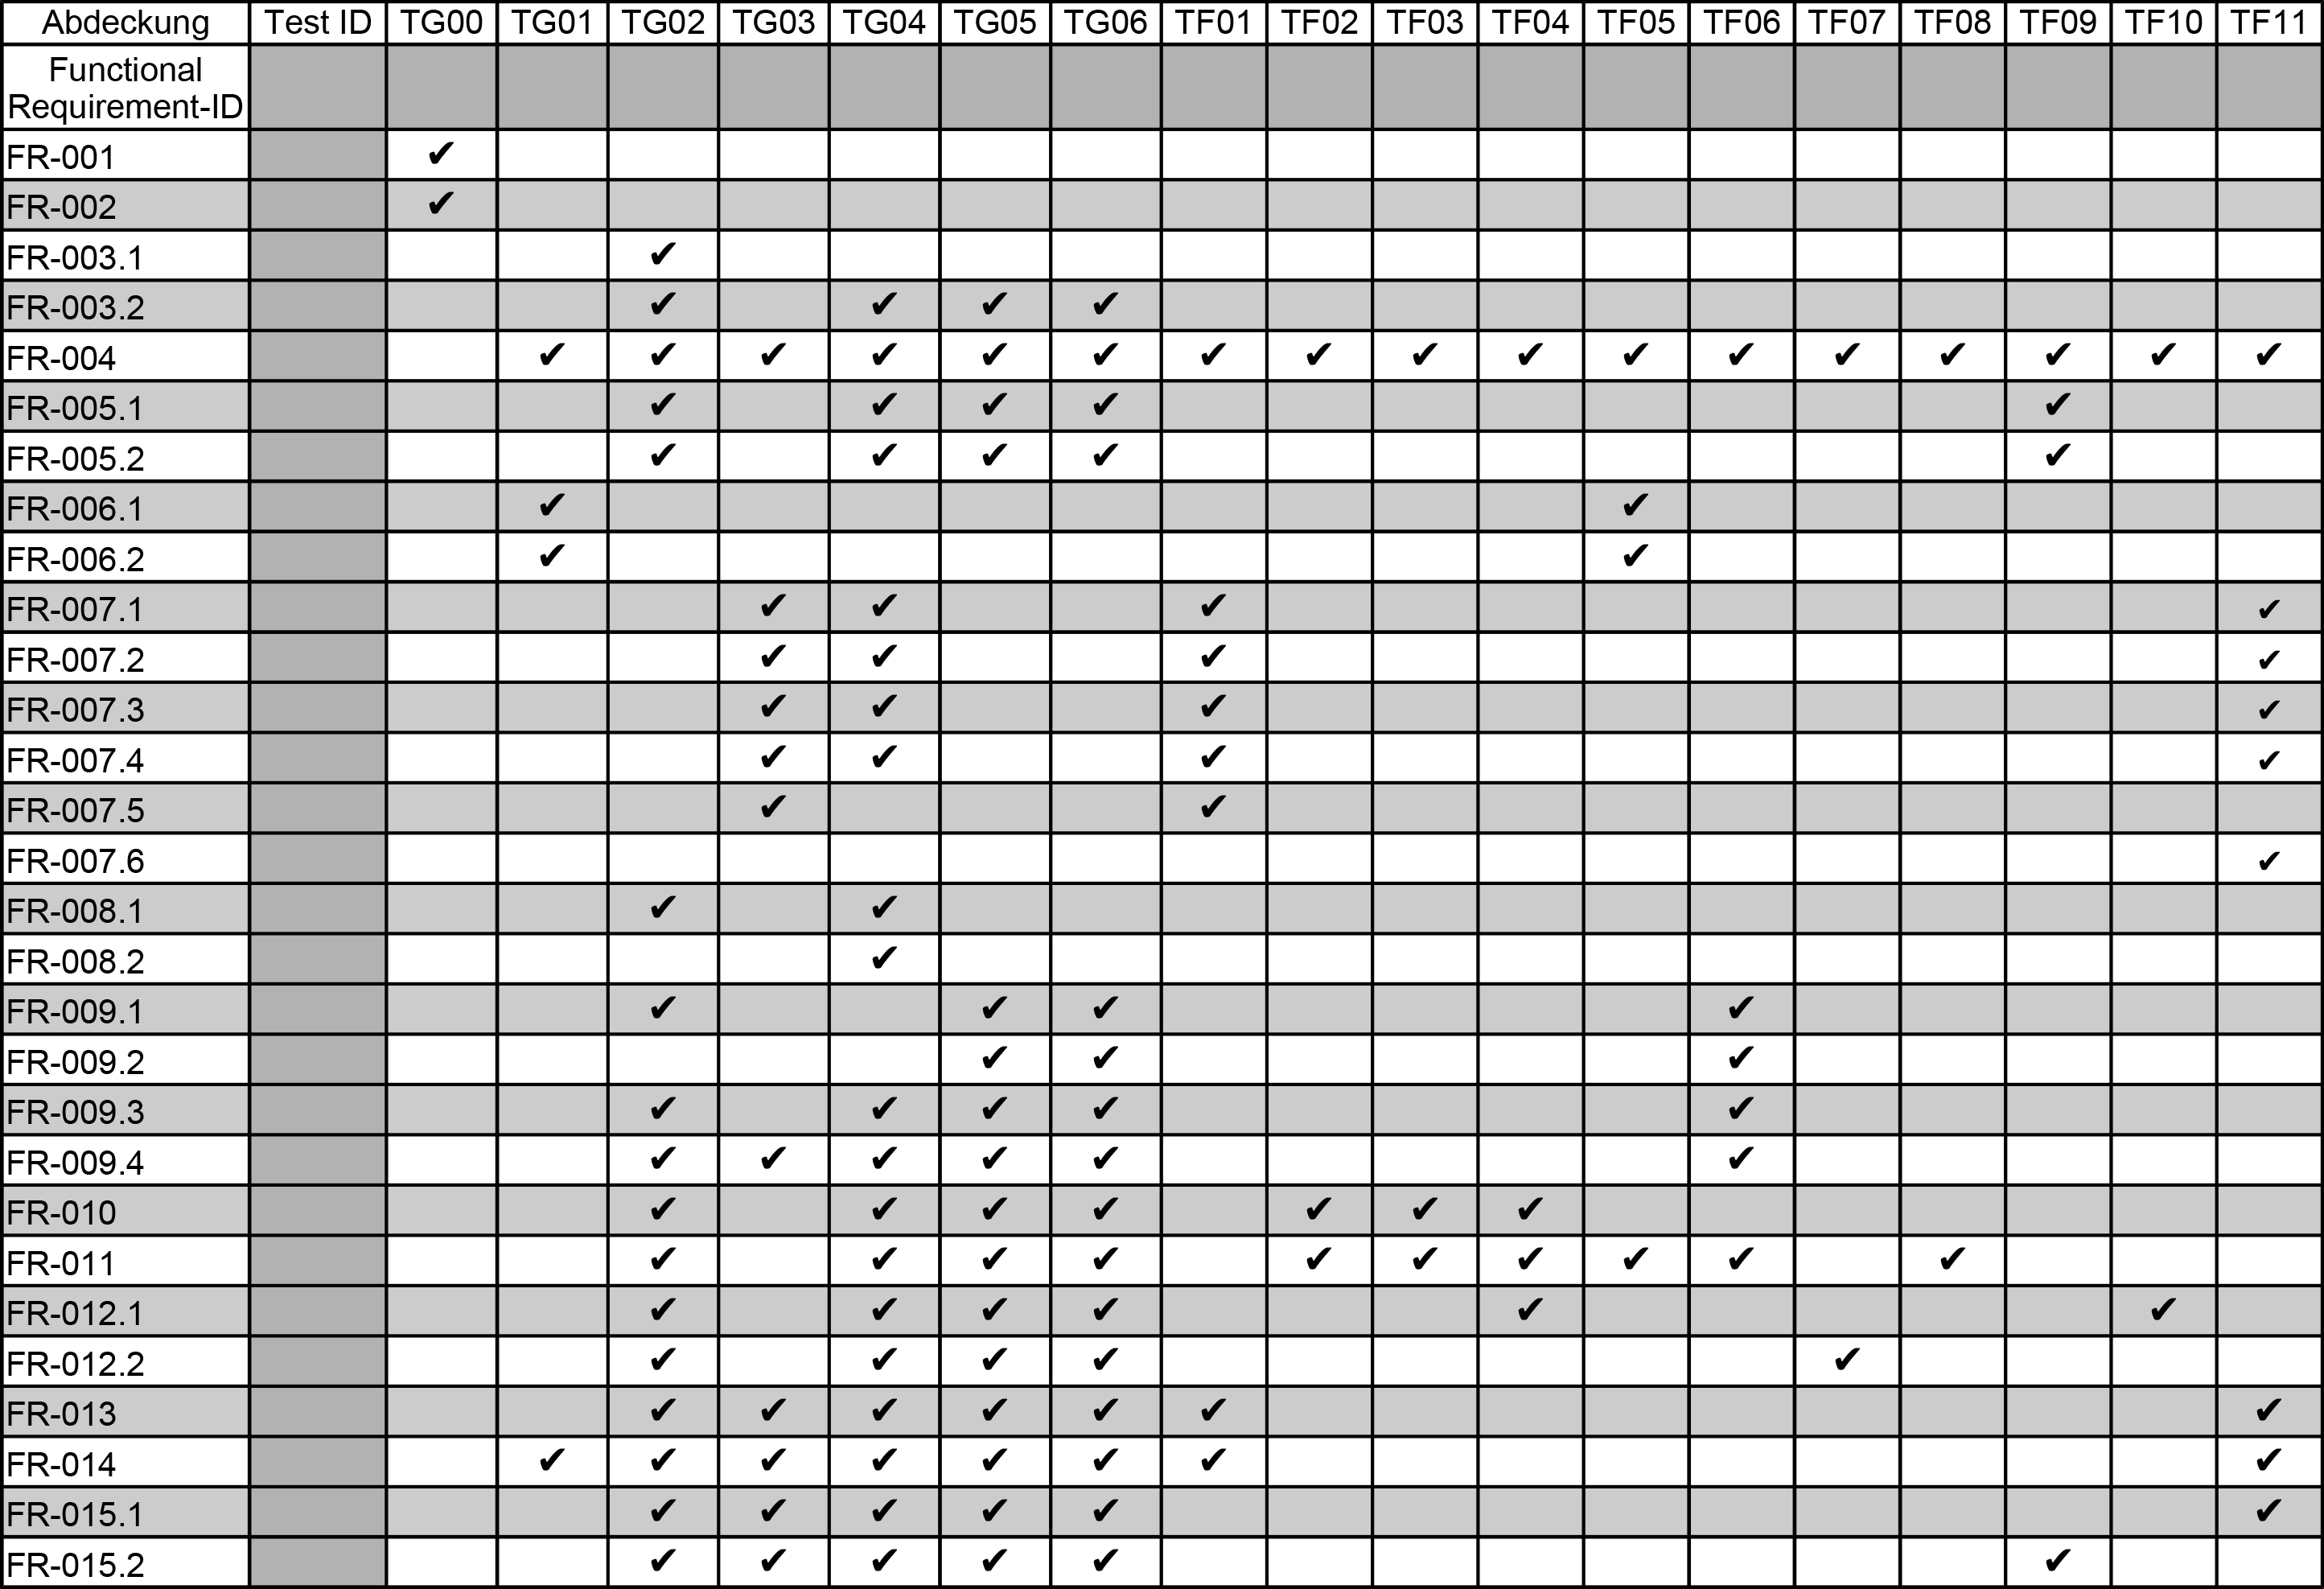
\includegraphics[angle=90,scale=0.305]{imgs/Req_Test_Abdeckung_1.png}
  \caption{Abdeckung der Functional Requirements [1/2]}
\end{figure}

% 8.5.4 Abdeckung der Functional Requirements [2/2]
\begin{figure}[p]
  \subsubsection{Abdeckung der Functional Requirements [2/2]}
  \centering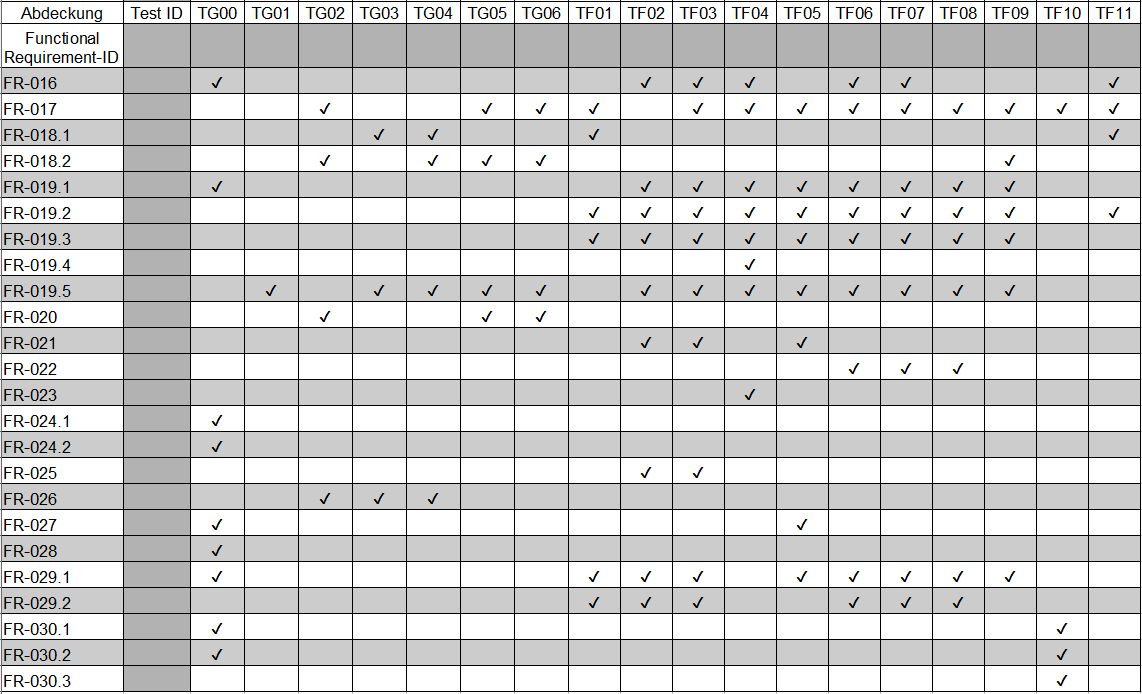
\includegraphics[angle=90,scale=0.305]{imgs/Req_Test_Abdeckung_2.png}
  \caption{Abdeckung der Functional Requirements [2/2]}
\end{figure}

% 8.5.5 Abdeckung der Non-functional Requirements
\begin{figure}[p]
  \subsubsection{Abdeckung der Non-functional Requirements}
  \centering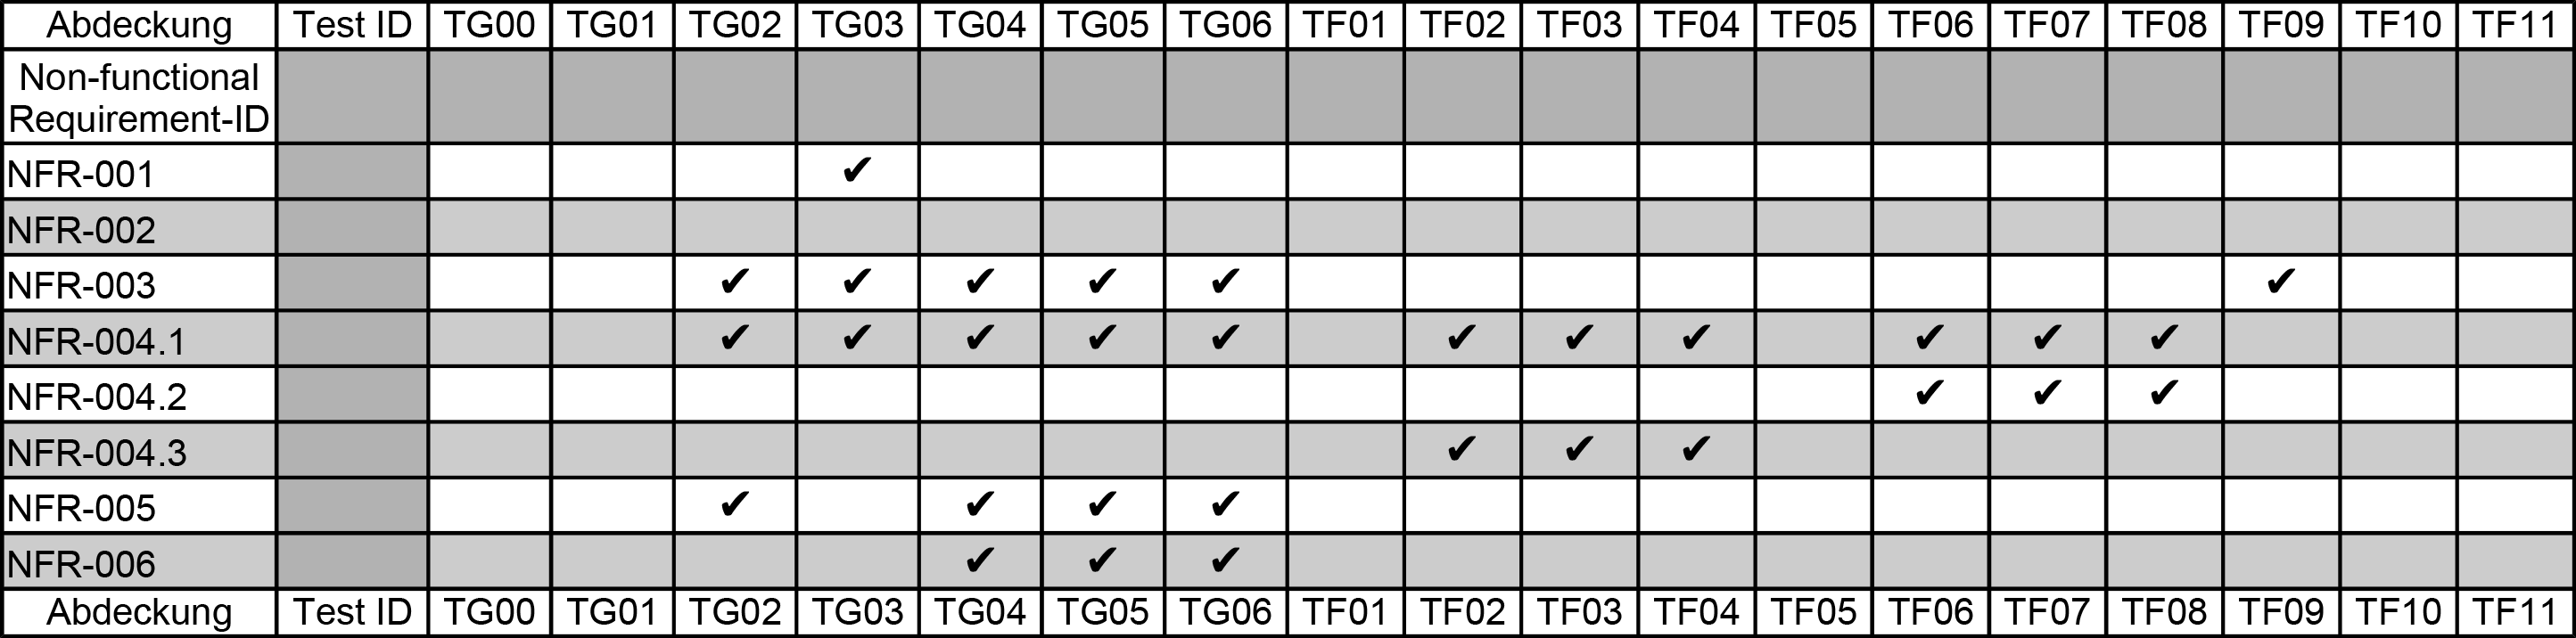
\includegraphics[angle=90,scale=0.305]{imgs/Req_Test_Abdeckung_3.png}
  \caption{Abdeckung der Non-functional Requirements}
\end{figure}

\newpage

% 8.6 Testprotokolle und Auswertungen
\subsection{Testprotokolle und Auswertungen}
04.11.2014: Testen der HAL, insbesondere der Sensorik\newline
Nachdem die korrekte Ansteuerung der Aktorik und die serielle Schnittstelle mit dem zweiten Milestone abgenommen wurde, wurde die Sensorik getestet. Es wurde beobachtet, dass der Höhensensor (korrekte) Messwerte liefert. Weiterhin wurde beobachtet, dass das Programm sich aufhängt, sobald ein Messwert geliefert bzw. ein Interrupt von der Sensorik ausgelöst wurde. Dies benötigt weitere Bearbeitung.\newline\newline
06.11.2014: Der Interrupt für die Sensorik funktioniert.\newline\newline
02.12.2014: Alle Tests wurden bestanden ohne Blinken der Ampel und Button LEDs, da diese zu diesem Zeitpunkt noch nicht implementiert waren. Getestet wurden Puck-Reihenfolge, Toleranzbereiche zu flacher Pucks, zu wendende Pucks auf B1 und deren Aussortierung auf B2 sowie das Warten von Pucks auf B1, wenn B2 belegt ist.\newline\newline
04.12.2014: Fehlerhafte Übergabe auf Band 2 bei folgender Werkstück Anordnung: Korrekt liegendes Werkstück, falsch liegendes Werkstück. Werkstück wird am Ende des Bandes gewendet.\newline\newline
04.12.2014: Fehlerhaftes Aussortieren von zu großen Werkstücken. Werkstück Anordnung: Korrekte Höhe, falsche Höhe.\newline\newline
08.12.2014: Der Fehler bei der Übergabe von Werkstücken wurde behoben. Dieser Fehler wurde ausgelöst durch einen Zustand der nicht korrekt bei dem Dispatcher
angemeldet war. Das hatte zur folge, das beim zurücklegen des Werkstückes die Lichtschranke durchbrochen wurde, jedoch das falsche Werkstück auf das Event sensitiv war.\newline\newline
08.12.2014: Ein Fehler beim Aussortieren wurde behoben. Dieser Fehler wurde ausgelöst dadurch, dass das zu kleine Werkstück (welches auf dem Band vor dem korrekten Werkstück liegt)
in die Lichtschranke der Weiche gekommen ist, jedoch nicht auf dessen Event sensitiv war. Das nachfolgende Werkstück mit korrekter Höhe war jedoch sensitiv auf dieses Event.
Das nachfolgende Werkstück hat die Weiche geöffnet, dadurch konnte dann das zu kleine Werkstück die Weiche passieren und den Weichenbereich verlassen. Die Weiche wurde geschlossen
und das Werkstück mit korrekter Höhe wurde aussortiert. \newline\newline
11.12.2014: Bei den Tests fiel auf, dass anstatt eines Blinkens ein Dauerlicht geleuchtet hat und dass am Ende von B2 keine gelbe Signalleuchte zum Entnehmen eines Pucks aktiv war. Dies erforderte jedoch nur kleine Änderungen, die vor Ort vorgenommen wurden. Bei den erneut ausgeführten Tests lief alles wie erwartet.\newline\newline
\newline\newline\textcolor{red}{\textbf{Das letzte Testprotokoll ist das Abnahmeprotokoll, das bei der abschließenden Vorführung erstellt wird. Es enthält eine Auflistung der erfolgreich vorgeführten Funktionen des Systems sowie eine Mängelliste mit Erklärungen der Ursachen der Fehlfunktionen und Vorschlägen zur Abhilfe}}

\newpage

% 9. Lessons Learned
\section{Lessons Learned}
Durch dieses Projekt haben wir viele Erfahrungen sammeln können. Sowohl bezüglich der Team-Organisation und Zusammenarbeit, als auch in der Entwicklung, Implementierung und Dokumentation eines größeren Projektes.\newline
Das Klima im Team war sehr angenehm. Getroffene Absprachen wurden eingehalten und jeder hat die ihm zugeteilten Aufgaben erledigt.\newline
Durch die Aufgabenverteilung konnte effizient und gleichzeitig an verschiedenen Aufgaben gearbeitet werden, was durchaus sinnvoll war, wenn wie bei diesem Projekt, Deadlines eingehalten werden mussten und entsprechend unter Zeitdruck gearbeitet wurde.\newline
Die Verteilung der Aufgaben hat allerdings dazu geführt, dass man wenig Einblick in die Arbeit der anderen bekommen hat und z.B. keine Architektur-Diskussionen geführt wurden, was Fehler von vornherein hätte vermeiden können. Als die Fehler schließlich aufkamen, war es teilweise schon zu spät, grundlegende Änderungen vornehmen zu können, sodass kleinere Workarounds notwendig wurden.\newline
Außerdem hat sich herausgestellt, dass eine Team-Organisation sehr schwierig ist, wenn die Wissensstände zu unterschiedlich sind.\newline
Des Weiteren wurde es als sehr anstrengend und schwierig empfunden, streng nach dem V-Modell vorzugehen. Diese Vorgehensweise hatten wir zu Beginn des Projektes zwar ausgewählt, es hat sich aber herausgestellt, dass die Verwendung des Scrumm- oder V-Modell-XT vermutlich besser gewesen wäre, weil damit eine gelockerte Vorgehensweise möglich ist.\newline
Weiterhin hat sich gezeigt, dass die Aufteilung eines großen Projektes in kleinere Milestones sehr hilfreich ist, um den Überblick zu behalten und gesetzte Deadlines einzuhalten. Die Deadlines sollten dabei schon früh angesetzt werden, damit die Aufgaben auch wirklich pünktlich fertig sind.\newline
Trotz Aufgaben-Splitting stellten wir fest, dass die Granularität der Commits bzw. Pushes auf GitHub immer noch teilweise zu grob war. Besonders bei der Bearbeitung von Binärdateien, an denen mehrere Personen gearbeitet haben. Hier ist es wahrscheinlich sinnvoller, die Commits und Pushes auf Grundlage von kleineren Paketen durchzuführen, was aber möglicherweise einer weiteren Fragmentierung der vorgegebenen Milestones bedarf.\newline
Etwas, worauf wir bei der Arbeit häufiger gestoßen sind, war die Tatsache, dass die Dokumentation, bzw. die UML-Diagramme nicht auf demselben Stand wie der Code waren. Daher sollte man, um Inkonsistenzen von vornherein zu vermeiden, dafür zu sorgen, dass bei Arbeiten am Code auch direkt alle dazugehörigen Dokumente mitbedacht werden.

\newpage

% 10. Glossar
\section{Glossar}
\begin{tabbing}
  Links Links Links \= Mitte \= Rechts \kill
  \textbf{Ampel, Signal:}    \> \> Warnsignalanlage der Förderbänder\\
  \textbf{Bohrung:}          \> \> Aushöhlung der Werkstücke\\
  \textbf{Förderband, Band:} \> \> Fließband des Festo-Typs\\
  \textbf{Interrupt:}        \> \> Asynchrone Nachricht einer Systemkomponente\\
  \textbf{Personal:}         \> \> Geschultes Personal, das die Werkstück-Sortieranlage bedient\\
  \textbf{QNX:}              \> \> Proprietäres Echtzeitbetriebssystem für eingebettete Systeme\\
  \textbf{Rutsche:}          \> \> Lagerplatz für aussortierte Werkstücke\\
  \textbf{Singleton:}        \> \> Modell zur Sicherstellung einer singulären Instanz\\
  \textbf{SEAP Simulation:}  \> \> Grafische Software-Simulation der Werkstück-Sortieranlage\\
  \textbf{Stakeholder:}      \> \> Gruppen, die mit der Anlage interagieren\\
  \textbf{Steuerung:}        \> \> Software, um die Hardware zu koordinieren\\
  \textbf{Stub:}             \> \> Programmcode, der als Platzhalter ein Verhalten / Hardware emuliert\\
  \textbf{V-Modell-XT:}      \> \> Standard für die Softwareentwicklung (Erweiterung des V-Modell)\\
  \textbf{Weiche:}           \> \> Schranke, um Pucks auszusortieren oder durchzulassen\\
  \textbf{Werkstück:}        \> \> Puck\\
\end{tabbing}


% 11. Abkürzungen
\section{Abkürzungen}
\begin{tabbing}
  Links \= Mitte \= Rechts \kill
  \textbf{B1:}   \> \> Sortierband 1\\
  \textbf{B2:}   \> \> Sortierband 2\\
  \textbf{DCLP:} \> \> Double-Checked Locking Pattern\\
  \textbf{FIFO:} \> \> First In First Out\\
  \textbf{FSM:}  \> \> Finite State Machine (Deterministischer Endlicher Automat)\\
  \textbf{GEME:} \> \> General Embedded Machine Engine\\
  \textbf{HAL:}  \> \> Hardware Abstraction Layer\\
  \textbf{IRQ:}  \> \> Interrupt Request\\
  \textbf{ISR:}  \> \> Interrupt Service Routine\\
  \textbf{RDD:}  \> \> Requirements and Design Documentation\\
  \textbf{WS:}   \> \> Werkstück\\
\end{tabbing}

\newpage

% 12. Anhänge
\section{Anhänge}

% 12.1 Coding Style: Google C++
\subsection{Coding Style: Google C++}

% 12.1.1 General Rules
\subsubsection{General Rules}
\begin{itemize}
  \item Use 2 spaces per indentation level.
  \item The maximum number of characters per line is 80.
  \item Never use tabs.
  \item Vertical whitespaces separate functions and are not used inside functions: use comments to document logical blocks.
  \item Header filenames end in \emph{.hpp}, implementation files end in \emph{cpp}.
  \item Never declare more than one variable per line.
  \item Ampersand {\&} binds to the \emph{type}, e.g., \emph{const std::string}\& \emph{arg}.
  \item Namespaces do not increase the indentation level.
  \item Access modifiers, e.g. \emph{public}, are indented one space.
  \item Use the order \emph{public}, \emph{protected}, and then \emph{private}.
  \item Use \emph{typename} only when referring to dependent names.
  \item Keywords are always followed by a whitespace: \emph{if (...), template \textless...\textgreater, while (...)}, etc.
  \item Always use \emph{\{\}} for bodies of control structures such as \emph{if} or \emph{while}, even for bodies consiting only of a single statement.
  \item Opening braces belong to the same line:
  \begin{lstlisting}
if (my_condition) {
  my_fun();
} else {
  my_other_fun();
}
  \end{lstlisting}
  \item Use standard order for readability: C standard libraries, C++ standard libraries, other libraries, your headers:
  \begin{lstlisting}
#include <sys/types.h>
#include <vector>
#include "some/other/library.hpp"
#include "myclass.hpp"
  \end{lstlisting}
  \item When declaring a function, the order of parameters is: outputs, then inputs. This follows the parameter order from the STL.
  \item Never use C-style casts.
\end{itemize}

% 12.1.2 Naming
\subsubsection{Naming}
\begin{itemize}
  \item Class names, constants, and function names are all-lowercase with underscores.
  \item Types and variables should be nouns, while functions performing an action should be "{}command"{} verbs. Classes used to implement metaprogramming functions also should use verbs, e.g., \emph{remove\_const}.
  \item Member variables use the prefix \emph{m\_}.
  \item Thread-local variables use the prefix \emph{t\_}.
  \item Static, non-const variables are declared in the anonymous namespace and use the prefix \emph{s\_}.
  \item Template parameter names use CamelCase.
  \item Getter and setter use the name of the member without the \emph{m\_} prefix:
  \begin{lstlisting}
class some_fun {
 public:
  // ...
  int value() const {
    return m_value;
  }
  void value(int new_value) {
    m_value = new_value;
  }
 private:
  int m_value;
};
  \end{lstlisting}
\end{itemize}

% 12.1.3 Headers
\subsubsection{Headers}
\begin{itemize}
  \item Each \emph{.cpp} file has an associated \emph{.hpp} file. Exceptions to this rule are unit tests and \emph{main.cpp} files.
  \item All header files should use \emph{\#define} guards to prevent multiple inclusion.
  \item Do not \emph{\#include} when a forward declaration suffices.
  \item Use \emph{inline} for small functions (rule of thumb: 10 lines or less).
\end{itemize}

\newpage

% 12.1.4 Breaking statements
\subsubsection{Breaking Statements}
\begin{itemize}
  \item Break constructor initializers after the comma, use four spaces for indentation, and place each initializer on its own line (unless you don't need to break at all):
  \begin{lstlisting}
my_class::my_class()
    : my_base_class(some_function()),
      m_greeting("Hello there! This is my_class!" ),
      m_some_bool_flag(false) {
  // ok
 }
other_class::other_class() : m_name("tommy"), m_buddy("michael") {
  // ok
}
  \end{lstlisting}
  \item Break function arguments after the comma for both declaration and invocation:
  \begin{lstlisting}
intptr_t channel::compare(const abstract_channel* lhs,
                          const abstract_channel* rhs) {
  // ...
}
  \end{lstlisting}
  \item Break before tenary operators and before binary operators:
  \begin{lstlisting}
if (today_is_a_sunny_day()
    && it_is_not_too_hot_to_go_swimming()) {
  // ...
}
  \end{lstlisting}
\end{itemize}

\end{document}

}
